% REMEMBER: You must not plagiarise anything in your report. Be extremely careful.
\documentclass{l4proj}

    
%==============================================================================
% Put any additional packages here
% You can add any packages you want, as long as it does not alter
% the overall format (e.g. don't change the margins or the reference style).
%

\usepackage{pdfpages} % if you want to include a PDF for an ethics checklist,
\usepackage{amsmath}
\usepackage{algcompatible}
\usepackage{wrapfig}

%
%


\begin{document}
%==============================================================================
%% METADATA
\title{Level 4 Project Report } % change this to your title
\author{Jan Wieczorek}
\date{September 14, 2018}

\maketitle

%==============================================================================
%% ABSTRACT
\begin{abstract}
    The aim was of the first stage of the project was to compare some aspects of the multidimensional scaling algorithms first presented by \citet{Chalmers96} and \citet{hyrid} and implemented in Python by \citet{2019} with the algorithm developed by \citet{squad}. as well as investigating the impact on the algorithms' performance of various additions and modifications. In the second stage ...
\end{abstract}

%==============================================================================
%% ACKNOWLEDGEMENTS
\chapter*{Acknowledgements}
% Enter any acknowledgements here. This is optional; you may leave this blank if you wish,
% or remove the entire chapter
%
% We give thanks to the Gods of LaTeX, who in their eternal graciousness, 
% have granted that this document may compile without errors or overfull hboxes.
%

%==============================================================================

% EDUCATION REUSE CONSENT FORM
% If you consent to your project being shown to future students for educational purposes
% then insert your name and the date below to  sign the education use form that appears in the front of the document. 
% You must explicitly give consent if you wish to do so.
% If you sign, your project may be included in the Hall of Fame if it scores particularly highly.
%
% Please note that you are under no obligation to sign 
% this declaration, but doing so would help future students.
%
\def\consentname {Jan Wieczorek} % your full name
\def\consentdate {10 March 2023} % the date you agree
%
\educationalconsent


%==============================================================================
\tableofcontents

%==============================================================================
%% Notes on formatting
%==============================================================================
% The first page, abstract and table of contents are numbered using Roman numerals and are not
% included in the page count. 
%
% From now on pages are numbered
% using Arabic numerals. Therefore, immediately after the first call to \chapter we need the call
% \pagenumbering{arabic} and this should be called once only in the document. 
%
%
% The first Chapter should then be on page 1. 

% PAGE LIMITS
% You are allowed 40 pages for a 40 credit project and 30 pages for a 
% 20 credit report. 
% This includes everything numbered in Arabic numerals (excluding front matter) up
% to but *excluding the appendices and bibliography*.
%
% FORMATTING
% You must not alter text size (it is currently 10pt) or alter margins or spacing.
% Do not alter the bibliography style. 
%
%==================================================================================================================================
%
% IMPORTANT
% The chapter headings and structure here are **suggestions**. You don't have to follow this model if
% it doesn't fit your project. Every project should have an introduction and conclusion,
% however.  If in doubt, your supervisor can give you specific guidance; their view takes precedence over
% the structure suggested here.
%
%==================================================================================================================================
\chapter{Introduction}

% reset page numbering. Don't remove this!
\pagenumbering{arabic} 

% You can use \todo{} to mark text that needs to be fixed. Anything inside will appear as highlighted 
% text in the final copy, and you will also get warnings when you compile (so you don't
% forget to take them out!)

\section{Overview and context}

With the continually increasing volume of data available in many academic as well as commercial contexts, there is a great demand for tools to efficiently process and extract useful information from multidimensional data sets. One interesting problem in this area is high-dimensional data visualisation. Since approaches such mosaic/pair plots or using shape, colour etc. to represent dimensions above 2, can only be useful for a small number of dimensions, this almost always involves some form of dimension reduction and generation of a 2D plot. 

As many state-of-the-art solutions to problems involving mapping high-dimensional inputs to lower-dimensional outputs make use of neural networks and deep learning, it is not surprising that a number of attempts have been made to apply these tools, notably Variational Autoencoder architectures, to visualisation \citep{ nn_vis1, nn_vis2, nn_vis3, nn_vis4, nn_vis5, nn_vis6, nn_vis7}. At least in some instances, however, the disadvantages of these approaches, while not unique to neural networks, can, nonetheless, include long processing times \citep{nn_vis5}, the need to tune multiple hyper-parameters that can radically alter the resulting 2D layouts \citep{nn_vis5, nn_vis6} and, potentially, lack of genralisablity as the network architecture might have to be altered and hyper-parameters readjusted for different data types. (examples to add)

The alternative, more popular, approach is to use one of the incredibly large number of available algorithms that do not require training a neural network. These can be, broadly, split into at least two major groups. The first - containing linear algorithms - includes one of the most commonly used dimensionality reduction procedure - Principal Component Analysis (PCA) \citep{pca}, which, while useful in visualisation, necessarily produces restricted, considerably simplified plots when treated as a standalone visualisation technique (see  Figure \ref{fig:init_demo}). Another linear method - classical Multidimensional Scaling (MDS) \citep{mds} was designed to preserve all pairwise distance relationships between the high-dimensional data points. It often outputs layouts of much better quality, representing both local and global structures fairly accurately. This however comes at the cost of processing time, which has the complexity of O(n\textsuperscript{3}) or O(n\textsuperscript{4}) for most classical MDS algorithms, making this technique impractical to use on large data sets.

Among non-linear methods, one class of iterative algorithms, which includes all three that are the main focus of this project - \citet{Chalmers96}, \citet{hyrid} and \citet{squad} introduces various heuristics and elements of stochasticity to the basic non-metric MDS procedure in an attempt to reduce its prohibitively large time complexity, without sacrificing layout quality. While largely successful in this task, like all visualisation algorithms based on MDS or other linear methods, these techniques tend to perform worse when the high-dimensional structures (manifolds) they aim to represent cannot be regarded as linearly or approximately linearly embedded in the observation space \citep{swissroll} - such as for example a world map rolled into a 3d swiss roll (see Section \ref{sec:non-linear}).  

The two most popular visualisation algorithms - UMAP \citep{umap} and especially t-SNE \citep{tsne} - as well as accelerated versions of the latter by \citet{barneshutsne} and \citet{fitsne}, are also non-linear. In contrast to the roughly equivalent focus on global and local structures of the MDS-based techniques, the above two algorithms tend to favour the latter at the expense of the former, requiring a suitable initialisation to achieve a reasonable degree of global structure preservation \citep{initialisationcritical} - Figure \ref{fig:init_demo}. At least due to their local focus the two algorithms should also be able to better handle nonlinear data manifolds \citep{swissroll}.


\begin{figure}[htb]
    \centering
    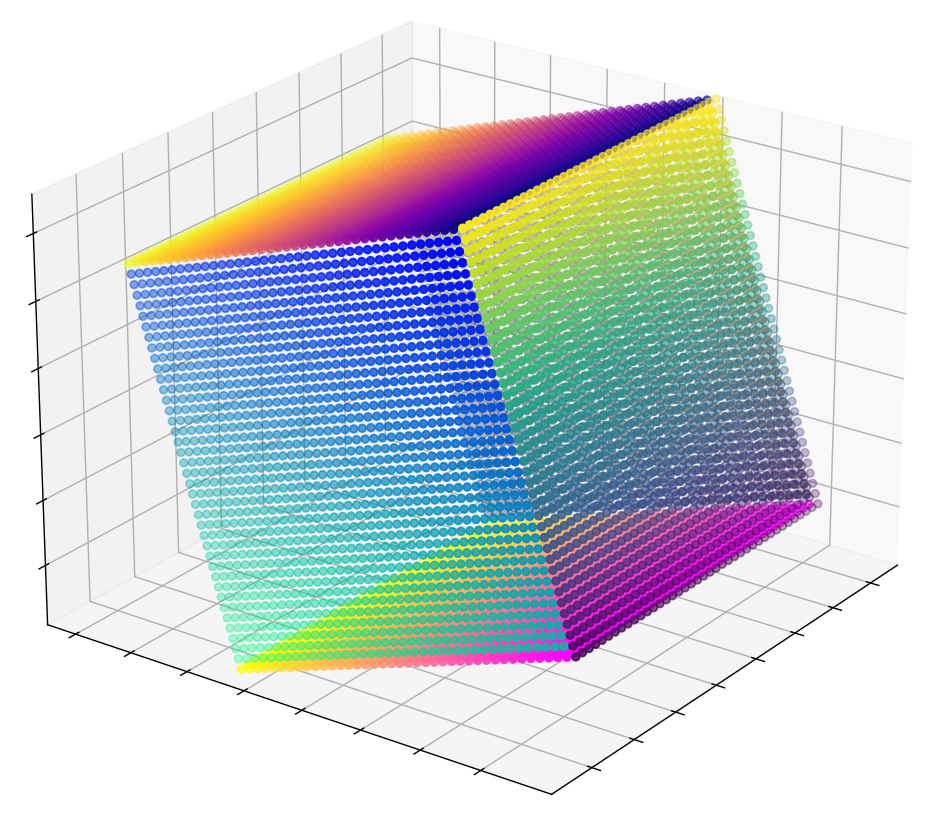
\includegraphics[width=0.3\linewidth]{images/cube/3dcube.png} \\
    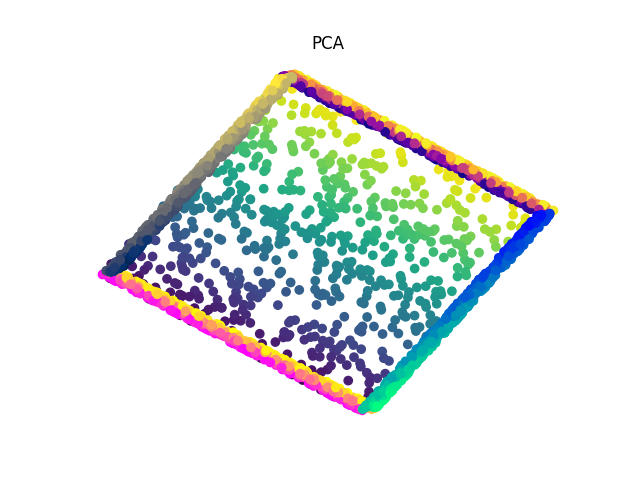
\includegraphics[width=0.3\linewidth]{images/cube/PCA.png}
    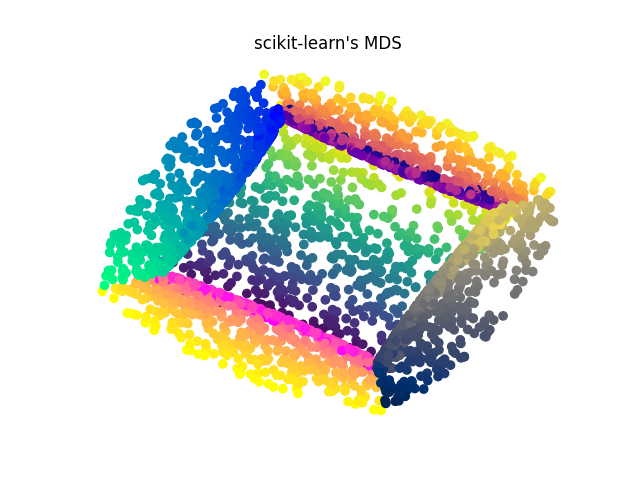
\includegraphics[width=0.3\linewidth]{images/cube/scikit-learn's MDS.png} 
    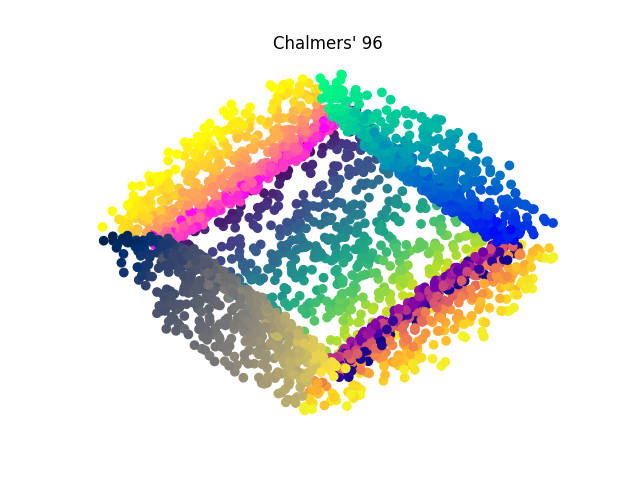
\includegraphics[width=0.3\linewidth]{images/cube/Chalmers' 96.png}\\
    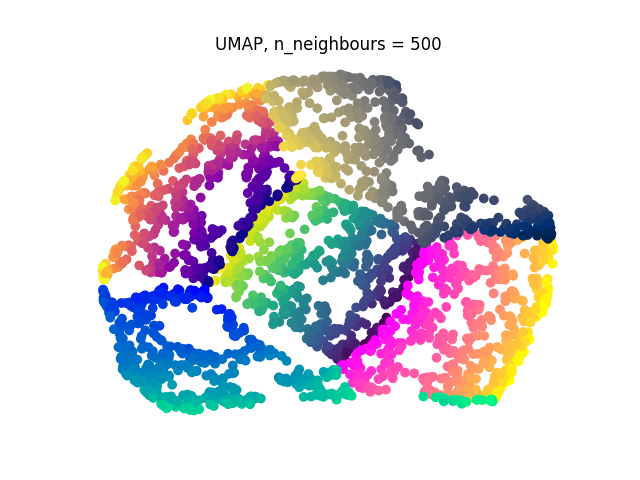
\includegraphics[width=0.3\linewidth]{images/cube/umap_cube.png} 
    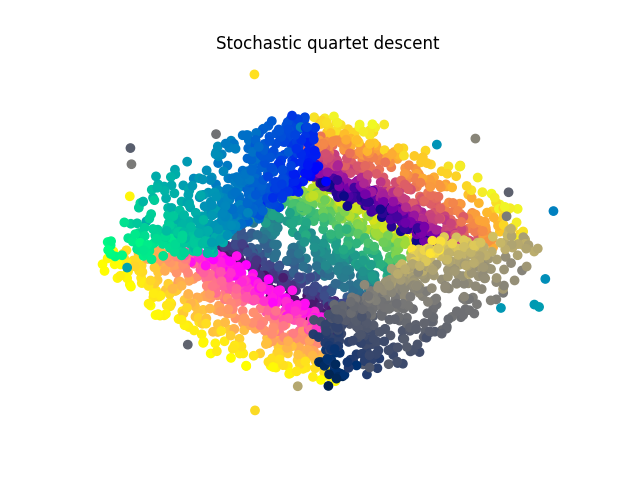
\includegraphics[width=0.3\linewidth]{images/cube/Stochastic quartet descent.png}
    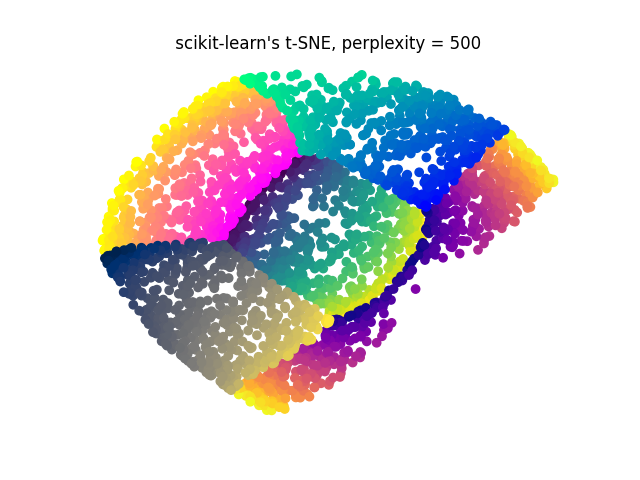
\includegraphics[width=0.3\linewidth]{images/cube/tsne_cube.png}\\

    \caption{An illustration (with reduced point density) of a set of 5x10\textsuperscript{4} non-overlapping, 3-dimensional points forming 5 faces of a cube and 2D embeddings produced by passing the same 3000 points sampled from the cube to various dimension reducing algorithms. UMAP was initialised with Laplacian Eigenmaps \citep{laplacian_eigen}, t-SNE and Stochastic quartet MDS with PCA. Chalmers' 96 MDS and scikit-learn's classical SMACOF MDS used random initialisations.
    }

    % use the notation fig:name to cross reference a figure
    \label{fig:init_demo} 
\end{figure}

\section{Motivation}

The aim of this project was jnjjfkjakbdsahbsdkajsb

Given the large number of parameters and settings governing the behaviour of each algorithm only the effect of more interesting or significant adjustments was formally tested and many others especially those whose effect was unambiguously detrimental were only investigated by manually running the algorithm on a few datasets. 
%==================================================================================================================================
\chapter{Background}

\section{Stress and other metrics.}

Like most MDS-based dimensionlity reduction methods the three considered algorithms use some variant of the loss function called "stress", first proposed by \citet{og_stress} and defined as: 

\begin{equation}
\label{tab:stress}
    Stress = \sqrt{\frac{\sum_{i<j}(\delta_{ij} - d_{ij})^2 }{\sum_{i<j}d_{ij}^2}},
\end{equation}    
where $\delta_{ij}$ is the high-dimensional distance between data points i and j and $d_{ij}$ is the distance between their low-dimensional representations. It is worth noting that, while enormously informative, such defined "stress" is not a perfect measure for assessing the quality of the 2D layouts, not least because this quality depends in part on the subjective judgement of the viewer and the purpose of visualisation (some systematic limitations are briefly illustrated in section 823492sss). This is one reason why it is common in  high-dimensional data visualisation literature to include qualitative evaluation of algorithms, often on simplified, synthetic data-sets, as part of the overall assessment of the algorithms' performance. For quantitative assessment a wide variety of, not infrequently custom designed, metrics is used. Many of those metrics highlight different aspects of the produced layouts. 

In this project three synthetic data sets were used: a 3d cube, a 3d globe and a 2d world map rolled into a 3d Swiss roll \footnote{"Swiss roll world map" idea and the bascic concept of how to generate it - by sampling points from continent images from: \url{https://github.com/NikolayOskolkov/tSNE_vs_UMAP_GlobalStructure}}. Apart from Stress the layouts were quantitatively evaluated by comparing their accuracy with k-NND algorithm - as in (reference to dig out) and by (nabsjnfanakan to add)

\section{Algorithms}

The values of all the algorithms' parameters which, unless explicitly stated otherwise, were used in all the experiments performed, are included in Appendix  
    
\subsection{\cite{Chalmers96}}
\label{chalmers96}

This algorithm relies on a spring force model to translate the high-dimensional distance structure of a data-set into two dimensions. To reduce the number of comparisons performed in the classical MDS, each data-point (or node) $i$ is assigned two non-intersecting sets of other nodes: a neighbour set $V_i$ and random sample set $S_i$. At each iteration a new sample is drawn for each node $i$ and the neighbour set $V_i$ is updated in case any closer neighbours are found. A force equal to the sum of all forces between the node i and each node j in either $S_i$ or $V_i$ is computed. Force between nodes i and j is defined as:
\begin{equation}
\label{tab:force}
        F_{ij} = ()
\end{equation}  
where $(k_{s}$ is a spring constant, is $(k_{d}$ a damping constant l is bla blah and $v_{ij}$ is the sum of the magnitudes of components of velocities of i and j in the direction of l. The implementation of the algorithm used in this project \citep{2019} did not include a spring force between each node and the 2D plane onto which the layout is projected, unlike in the original paper \citep{Chalmers96}. As noticed by \citet{2019} in this implementation the 2D layouts stop evolving after around 100 (much smaller than N) iterations for most data-sets and thus, since the sizes of $S_i$ and $V_i$ are kept constant, the algorithm effectively operates in linear time rather than $O(N^2)$ as described by \citet{Chalmers96}. 

The role of $k_{d}$ is to prevent the system from becoming unstable (see section 412311) by reducing the overall force on a node. Nonetheless it was found that best results where produced when $k_{d}$ was set to zero and $k_{s}$ was directly decreased instead, as in the original implementation by \citet{2019}. Similarly, initial experiments revealed that  thus this setting was also left unchanged. Finally,  again as in the original implementation, for simplicity, the integration step is set to one, so that force, velocity and position update of a node become equal. 

\subsection{\cite{hyrid}}

Here the runtime of \citet{Chalmers96} is further reduced by only applying the full layout algorithm on a $\sqrt{N}$ subset of the dataset, interpolatin the remaining datapoints into the layout and finally gghhg. During interpolation stage for each datapoint not yet placed on the 2D layout ghhgg. Further details are discussed in (ghghjhu). As before since the original specification \citep{Chalmers96} assumes to run in $O(n^2)$ time this modification originally reduced the time complexity to $O(n\log n)$ but in \citet{2019} implementation it reduces it to a shorter linear time.

\subsection{\cite{squad} - Stochastic Quartet Descent MDS (SQuaD)}

This is, in many ways, a similar approach to reducing the time complexity of classical MDS to that employed by \citet{Chalmers96}. Instead of using a heuristic of spring forces based on $V_i$ and $S_i$, however, at each iteration this algorithm randomly partitions the dataset into groups of four (quartets) and updates the low dimensional position of each datapoint in a quartet simultaneously, directly based on the gradients of the stress function calculated for the quartet, which is defined as:
\begin{equation}
\label{tab:quartet_stress}
    Stress_{quartet} = \sum_{a\, =\, 1}^{3} \sum_{b\, =\, a\, +\, 1}^{4} (\delta_{ij}^{\,r} - d_{ij}^{\,r})^2,
\end{equation} 
Here $\delta^{r}$ and $d^{r}$ are matrices of relative, that is normalised by the sum of all distances in the quartet, respectively high- and low-dimensional distances between datapoints i and j. The total stress of the layout is then defied as the average of all quartet stresses. Since the number of iterations required for convergence is around 500 and independent of N (?) this is, again, a linear time algorithm. The code provided by the authors \footnote{ \url{https://github.com/PierreLambert3/SQuaD-MDS}} served as the starting point for the implementation used in this project. During the initial exploration of the parameter space of the algorithm it was found that the layouts produced improved slightly when the learning rate was not decayed at every iteration, as in the original code, but maintained constant.


%==================================================================================================================================
\chapter{Design}



Appendix \ref{appendix a}

%==================================================================================================================================
\chapter{Experiments}

\section{Measurement challenges and the scope of comparisons}
\label{sec:measurements and scope}

A comparison between any two high-dimensional data visualisation algorithms could focus on many aspects of their performance. One such important aspect is memory use. However, despite the existence of various measurement tools for Python, obtaining accurate figures is not easy \footnote{ \url{https://pythonspeed.com/articles/measuring-memory-python/}}. Some tools only measure RSS memory use, others limit themselves to memory blocks allocated by Python interpreter itself, not including those used by libraries written in different languages, while yet others are only available for specific platforms, such as Linux. This is why early on in the project it was decided that memory use measurement will not be a major focus of this work.

More broadly, given that the algorithm implementations by \citet{2019} and \citet{squad} were written using different styles, the sheer number of possible tiny alteration which might or might not improve efficiency of either of them and the fact that the algorithms seemed to be broadly equally efficient in their existing implementations; it seemed that the project could take at least three main approaches to comparing the algorithms.

\begin{itemize}
\item  First, in order to make the comparison between SQuaD and the spring forces algorithms implemented by \citet{2019} fairer, would involve completely rewriting the code  for either of them - e.g. the latter to use a popular Python acceleration library Numba\footnote{ \url{https://numba.pydata.org/}}.

\item  Second would explicitly focus on making both algorithms' implementations as efficient as possible, perhaps with the restriction of only using Python API and Python libraries, and then measuring their relative performance.

\item  Third would generally only alter the high-level logic of the algorithms, focus on the quality of the produced embedding/layouts rather than efficiency and use the existing implementations as baselines.
\end{itemize}

It was decided that the last option would be the most interesting and useful one to take.

\section{Data sets}
\label{sec:datasets}

Include dimessions!!

Numerous data sets were considered for use in this project but only several are included in the formal comparisons between algorithms. These are (each (N,D) tuple indicates the size - N, and the number of dimensions -D ): a randomly sampled subset of MNIST\footnote{\url{https://scikit-learn.org/stable/modules/generated/sklearn.datasets.fetch_openml.html}} (7000, 784), a similarly reduced Fashion MNIST data set\footnote{\url{https://github.com/zalandoresearch/fashion-mnist}} (7000, 784), and Coil20 data set\footnote{\url{https://www.cs.columbia.edu/CAVE/software/softlib/coil-20.php}} (1440, 1024) with dimensions reduced as by the authors of SQuaD\footnote{ \url{https://github.com/PierreLambert3/SQuaD-MDS}}. All three of the above are commonly used in training various image processing systems. Further, the experiments used a data set of single-cell RNA sequencing data obtained from the mouse cortex\citet{mouse_cortex} (Mouse cortex scRNA), again, as provided by the authors of SQuaD \citep{squad} who used the pre-processing described in \citet{mouse_cortex_preprocess}. Finally, a synthetic data set of 3d points corresponding to the positions of all the major landmasses on a globe (Globe) - (7000, 3). To create this data set code from Nikolay Oskolkov\footnote{\url{https://github.com/NikolayOskolkov/tSNE_vs_UMAP_GlobalStructure}} was used to create 2D images of all the continents with Cartopy \footnote{\url{https://scitools.org.uk/cartopy/docs/latest/}} and the Platee Caree projection. Custom code was the written to sample points from those images and project the sampled points onto a sphere using an inverse Platee Caree projection. 
 . 


\section{Confirming the algorithms' time complexity}

\section{Stress Vectorisation with Numpy}

ADD SPEC!!!

\begin{figure}[h]
    \centering
    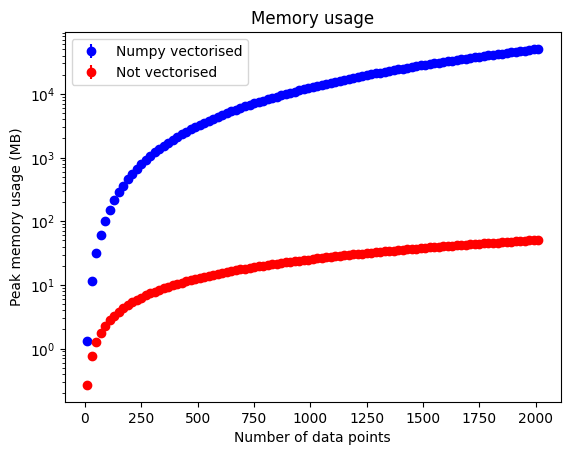
\includegraphics[width=0.4\linewidth]{images/stress_vectorised/memory.png}
    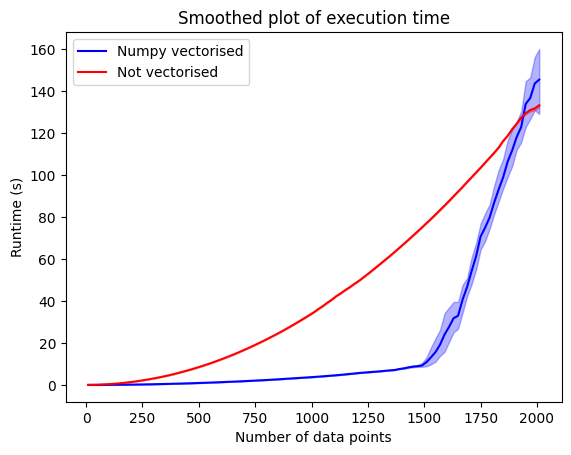
\includegraphics[width=0.4\linewidth]{images/stress_vectorised/time.png} 
 
    \caption{Peak memory usage and a smoothed (with a running mean of 5) plot of execution time for Stress (\ref{tab:stress}) calculation. Each measurement for both plots was performed three times but only for Numpy vectorised execution time some variability becomes visible - the shaded area corresponds to the range between the max and min measurement, whereas the line represents the mean. Stress was computed for data set sizes from 10 to 2010 with a step of 20.
    }

    % use the notation fig:name to cross reference a figure
    \label{fig:stress_vectorised} 
\end{figure}

Despite the aforementioned lack of specific focus on efficiency, one aspect of the computations performed where a decrease in execution time presented some benefits was calculation of Stress (\ref{tab:stress}) of a layout. Stress calculation is an expensive $O(n^2)$ operation which if performed periodically during layout creation tended to take up the majority of runtime. This was especially cumbersome when performing numerous quick, informal, tests on data sets of (further) reduced  sizes. Thus the original implementation using the \emph {itertools} library\footnote{ \url{https://docs.python.org/3/library/itertools.html}} and a Python loop, was rewritten with Numpy\footnote{ \url{https://numpy.org/}} as in Listing \ref{lst:vectorised_stress}. This provided an interesting opportunity to compare resource use by the two methods. The experiment was performed on a machine with 32.0 GB (31.7 GB usable) physical RAM, using the Python tool \emph {tracemalloc} which, as related to the discussion in Section \ref{sec:measurements and scope}, does track memory allocated to Numpy{\footnote{\url{https://numpy.org/devdocs/release/1.13.0-notes.html}}. As expected the vectorised method used much more - up to 3 orders of magnitude - memory but was significantly faster. However at the level of memory usage of around 26 GB the Numpy method performance begins to degrade rapidly - which must be caused primarily by the increasing use of swap space - until finally at levels above around 40GB an insufficient memory exception is thrown. In such cases, in this project, the original calculation method is used as a fallback.

\begin{lstlisting}[language=python, float, caption={Python code to calculate vectorised Stress. A "distance\_function" retruns a norm of a numpy array (1st parameter) calculated along the specified axis (2nd parameter).}, label=lst:vectorised_stress]
def vectorised_stress(data: np.ndarray, ld_positions: np.ndarray, distance_function: Callable):
    
    hd_dist = distance_function(data[:,:,None] - data[:,:,None].T, 1)
    ld_dist = distance_function(ld_positions[:,:,None] - ld_positions[:,:,None].T, 1)
    numerator = np.sum((hd_dist - ld_dist)**2)
    denominator = np.sum(ld_dist**2)
    if denominator == 0:
        return np.inf
    else:
        return np.sqrt(numerator/denominator)
    
\end{lstlisting}


\section{Comparing \cite{Chalmers96} algorithm and SQuaD }}
\subsection{Choosing the number of iterations}

\section{Varying neighbour and sample set sizes for \cite{Chalmers96}}
\section{Stochastic "N-tet" Descent MDS}

In this experiment the effect of changing the original size  (four) of the base unit used for layout creation by SQuaD was explored. Thus the SQuaD algorithm adapted for an arbitrary unit size greater than 3 was named Stochastic "N-tet" Descent (SNeD) - where "n-tet" stands for: trio, quartet, quintet, sextet and so on.  

Taking the partial derivative of one part of the loss function sum (\ref{tab:quartet_stress}) adapted for an arbitrary n-tet size $k$, with respect to one of the two dimensions on the 2D layout, e.g. $x$, of the $q^{th}$ point in the n-tet, results in: 

\begin{equation}
\label{tab:adapted quartet stress}
    \frac{\partial (\delta_{ij}^{\,r} - d_{ij}^{\,r})^2}{\partial x_q} = \frac{2}{\sum_{i<j}d_{ij}}(\delta_{ij}^{\,r} - d_{ij}^{\,r})\left(\frac{\partial d_{ij}}{\partial x_q} +  \frac{\partial \sum_{i<j}}{\partial x_q}d_{ij}^{\,r}\right) 
\end{equation}

\begin{center} which can be further reduced and re-arranged to: \end{center}

\begin{equation}
\label{tab:adapted quartet stress expanded}
     \frac{2}{\sum_{i<j}d_{ij}}(\delta_{ij}^{\,r} - d_{ij}^{\,r}) \left(\frac{I_{qi}(x_q - x_j) + I_{qj}(x_q - x_i)}{d_{ij}}  -  d_{ij}^{\,r} \sum_{b\in\{1,...,k\}\setminus q} \frac{x_q - x_b}{d_{qb}} \right), 
\end{equation} 

as in \citet{squad}. $\delta$ and $d$ represent the matrices of respectively, high- and low-dimensional distances between n-tet points while $\delta^{r}$ and $d^{r}$, as before, are their relativized equivalents. The identity matrix $I$, of dimensions $k$x$k$, provides a concise way of representing how the formula changes depending on whether $q$ is equal to either $i$ or $j$. 

While adapting the gradient formula for an arbitrary $k$ was trivial, this modification required substantial changes to the code base. In the original version, quartet distances and all parts of the gradient sum were computed manually, which allowed for easy application of Numba\footnote{ \url{https://numba.pydata.org/}} acceleration. All these calculations were rewritten from scratch, and, as far as possible, vectorised with variable-size Numpy arrays. Care was taken to still enable Numba acceleration for all operations, though this was not achieved for the computation of distances between n-tet points. 

\begin{figure}
    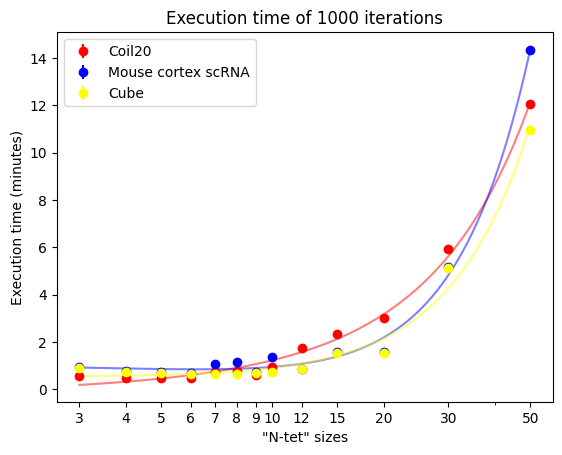
\includegraphics[width = 0.45\linewidth]{images/n-tet layouts/summary/time.png}
    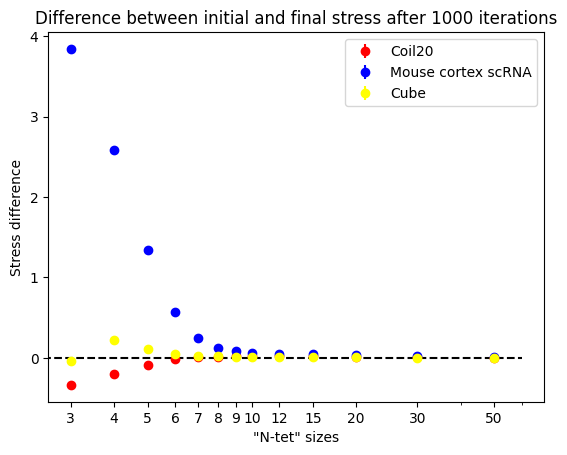
\includegraphics[width = 0.45\linewidth]{images/n-tet layouts/summary/stress.png}

    \caption{"N-tet" experiment results. The algorithm was re-run 6 times for each n-tet size but the consistency of measurements causes the error bars  not to be visible at this scale. Note the negative stress difference for the Coli20 dataset, and for the Cube dataset with n-tet size = 3, on the right.}
    \label{fig:ntet_summmary}
\end{figure}

The results of running the algorithm with different n-tet sizes $k$ are shown in Figure \ref{fig:ntet_summmary}. It is worth noting that the final Average N-tet Stress - ANS (adapted \ref{tab:quartet_stress}) did not appear to be an informative metric to compare layouts produced with different n-tet sizes, as it seemed to always decrease with increasing $k$. Given the implementation used in this project, this was tested by rerunning the SNeD algorithm on the same random layout with different $k$, all position updates set to zero, and comparing the final ANS. In consequence the classical Stress (\ref{tab:stress}) was the main comparison metric. 

The main finding was that for all datasets used, the algorithm made very little progress beyond the layout with which it was initialised as $k$ (n-tet size) approached values higher than 12. This is reflected in the Stress measurements shown in Figure \ref{fig:ntet_summmary} (see also Appendix \ref{appendix b}).

Interestingly, unlike for other data sets tested here, when run on Coli20 with $k$ values below 8, SNeD increased the Kruskal stress as it run. This behaviour was not exclusive to Coil20 but did not immediately appear to be consistently related to any single, easily identifiable feature of a dataset. The stress decreased as expected for a data set with 20531 dimensions\footnote{\url{https://archive.ics.uci.edu/ml/datasets/gene+expression+cancer+RNA-Seq}} - even greater number than that of Coil20 and while it increased for Fashion MNIST, which like Coil20 contains real-object images, it did so for a very different data set type - Flow Cytometry\footnote{\url{https://flowrepository.org/id/FR-FCM-ZZ36}} (number of dimensions 17) as well .

Regardless of Stress measurements, a simple qualitative, visual inspection of the layouts produced ( Appendix \ref{appendix b}) might suggest that 

\section{Non-linear data manifolds and comparison with t-SNE and UMAP}
\label{sec:non-linear}

Given the, at least to some extent, non-MDS-like behaviour of SNeD mentioned in the previous section, it was particularly interesting to check how the MDS-based algorithms considered in this project perform on data sets containing non-linear data manifolds, such as objects rolled into a "swiss-roll" \citep{swissroll}, as compared to the popular visualisation alternatives of UMAP and t-SNE. 



\section{Nesterov's momentum}

Nesterov's momentum is a method of accelerating the convergence of gradient descent first proposed by \citet{og_nesterov} and popularised by \cite{nesterov_hinton}. The process of updating the position of a point $x$ with Nesterov's momentum can be described by the following equations:


\begin{gather}  
    v_{t + 1} = \mu v_t  - \varepsilon \nabla f(x_t + \mu v_t) \\
    x_{t + 1} = x_t + v_{t+1}
\end{gather} 
Where $x_t + \mu v_t$ is the projected position update using change $v_t$, $\mu$ is the momentum and $\varepsilon$ is the learning rate. Thus, in contrast to classical momentum \citep{classical_momentum} this mechanism "looks ahead" by using the gradient of the projected position of x.

The idea of using Nesterov's momentum to attempt to accelerate SQuaD was described in an extended version of the SQaD paper \citep{squad} by the authors themselves. It was not, however, included in the code\footnote{ \url{https://github.com/PierreLambert3/SQuaD-MDS}} on which the implementation used in this project is based.

To test the effect of applying Nesterov's momentum to SQuaD's gradient descent, as before, the algorithm was re-run 20 times for each of the datasets (Section \ref{sec:datasets}) and each condition (momentum turned on and off). For each run, the number of iterations needed to reach a certain preset Average N-tet Stress (ANS) level for a given dataset, was recorded. The value of $\mu$ was chosen experimentally to be 0.6 in a arbitrary trade-off between the effect size and performance. $\varepsilon$  was left unchanged from the SQuaD's default (see Appendix  \ref{s}). Again, as before, Welch's t-test was conducted on the collected data.


% Please add the following required packages to your document preamble:
% \usepackage[table,xcdraw]{xcolor}
% If you use beamer only pass "xcolor=table" option, i.e. \documentclass[xcolor=table]{beamer}
\begin{table}[h]
\begin{tabular}{|
>{\columncolor[HTML]{DAE8FC}}l |c|c|c|c|}
\hline
\multicolumn{1}{|c|}{\cellcolor[HTML]{CBCEFB}Dataset} &
  \cellcolor[HTML]{CBCEFB}\begin{tabular}[c]{@{}c@{}}Mean iterations\\ with Nesterov's \\ momentum\end{tabular} &
  \cellcolor[HTML]{CBCEFB}\begin{tabular}[c]{@{}c@{}}Mean iterations\\ without Nesterov's\\ momentum\end{tabular} &
  \cellcolor[HTML]{CBCEFB}\begin{tabular}[c]{@{}c@{}}Target\\ ANS\\ value\end{tabular} &
  \cellcolor[HTML]{CBCEFB}\begin{tabular}[c]{@{}c@{}}Welch's t-test's \\ p-value\end{tabular} \\ \hline
Mouse cortex scRNA & 423 (SD 50.7) & 364 (SD 28.5) & 0.0129  & 5.87e-05 \\ \hline
Coil20             & 207 (SD 9.1)  & 127 (SD 8.2)  & 0.015   & 2.72e-27 \\ \hline
Globe              & 138 (SD 8.9)  & 110 (SD 1.4)  & 0.0019  & 5.63e-12 \\ \hline
Fashion MNIST      & 357 (SD 11.7) & 263 (SD 11.6) & 0.01128 & 2.38e-25 \\ \hline
MNIST              & 451 (SD 14.1) & 308 (SD 13.4) & 0.0218  & 2.62e-29 \\ \hline
\end{tabular}
\caption{Table summarising the results of Welch's t-test p-values values, with the alternative hypothesis of the Nestorov's momentum's mean being greater, performed for samples of 20 runs of the SNeD algorithm (n'tet size 4)) for different data sets. For each run the number of iterations needed to reach a preset Average N-tet Stress (ANS) level was recorded.}
\label{table:nesterov}
\end{table}

The results are summarised in Table \ref{table:nesterov}. They unambiguously show that for the data sets and parameter values used here, rather than improving convergence, the application of Nesterov's momentum impairs the algorithm's performance. 

\begin{wrapfigure}{l}{0.5\textwidth}
    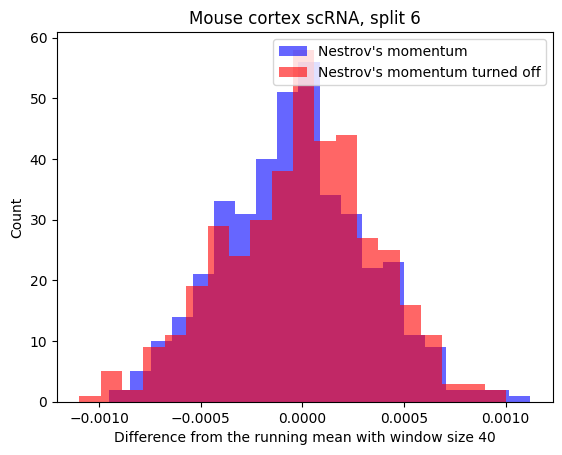
\includegraphics[width=0.48\textwidth]{images/nesterov/histogram.png}

  \caption{Histogram of differences between ANS measured at every iteration and the running mean for one section (or split) of the generation metrics graph (such as those in Figure !!!n-tet gen!!! ). All other datasets and sections had similar histograms as no clear, consistent difference in variances was observed.}
\label{fig:histogram}
\end{wrapfigure}

In fact, for several data sets, Nesterov's momentum, at least initially, increased the ANS instead of speeding up its descent (see Figure \ref{fig:nestrov}). Surprisingly, there did not appear to be any notable, consistent difference in the variance of ANS from one iteration to another between the two conditions (see Figure \ref{fig:histogram}).

 To exclude the possibility that these results were caused by a simple bug, as in all other case in this project, Pytests were used. These tested both the correct application of the Nesterov's momentum formula (by comparing the position updates computed by the algorithm to manual calculation) and the expected behaviour of Nesterov's mechanism (the values of $v_t$ continually increase if moving along the same direction keeps reducing the loss function) - however no bugs were found. 

 A more thorough investigation would be needed to identify the causes of the observed behaviour. Nonetheless, the obtained results seem to indicate that Nesterov's momentum does not improve the performance of the SQuaD algorithm.

\begin{figure}
    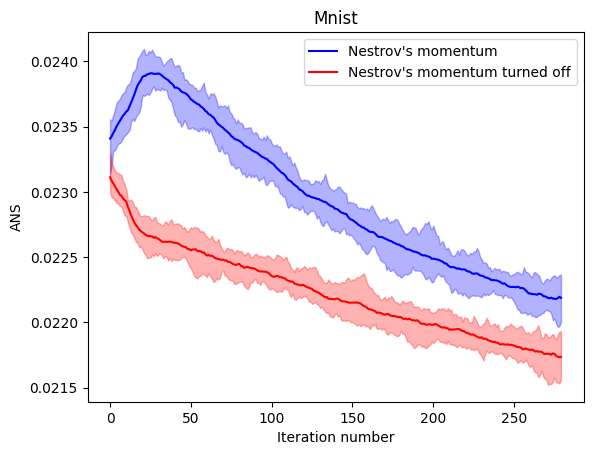
\includegraphics[width = 0.45\linewidth]{images/nesterov/mnist.png}
    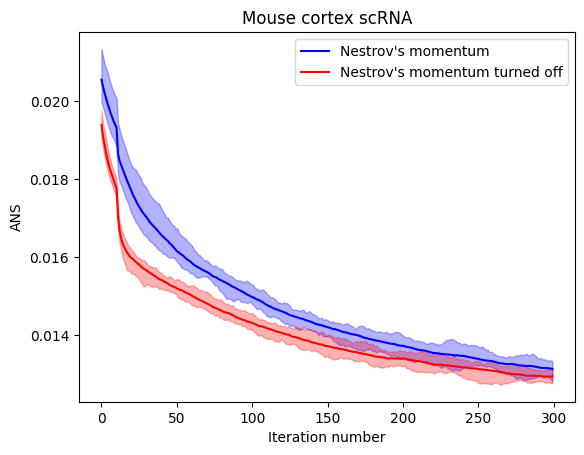
\includegraphics[width = 0.45\linewidth]{images/nesterov/rna.png}

    \caption{Graphs of the running means of window size 20 of ANS values collected during 20 layout generations for each condition. The solid line represents the mean of the means and the shaded are their range. ANS was measured on every iteration.}
    \label{fig:nestrov}
\end{figure}


\section{Applying k-NN descent algorithm to \cite{Chalmers96}}

In this experiment the \cite{Chalmers96} algorithm was modified to use unchanging neighbour sets pre-computed with the \citet{knnd} algorithm as implemented in Python by Leland McInnes\footnote{\url{https://github.com/lmcinnes/pynndescent}}, instead of updating them at each iteration.




\section{"Sudden layout collapse"}

During the exploration of the parameter space of the (slightly modified) \citet{2019} implementation of the \citet{Chalmers96} algorithm it became apparent that for values of the spring constant above a certain threshold, the layout "collapsed" to a single tight cluster or a thin line with some outlier points scattered around. At the same time, during layout creation the average speed of data points (or equivalently average force applied) rose exponentially. The threshold also appeared to be inversely proportional to the combined size of $V$ and $S$ (see Section \ref{chalmers96}). This behaviour was clearly noticed by \citet{2019}, despite not being mentioned in the dissertation, as his code introduced an appropriate scaling factor for the spring constant. 

A careful investigation with small, synthetic data sets confirmed that 
the collapse occurred due to the fact that at each iteration the updates of the 2D positions of the data points were computed as follows. Here, $P$ is the set of all 2D points, $F_{pq}$ is the force directed from $p$ to $q$, $V_{p}$ and $S_{p}$ are, respectively, the neighbour and sample sets of point $p$ and finally, $p_{u}$ and $q_{u}$ are used to store the cumulative force on points $p$ and $q$.

\begin{algorithmic}
\FOR { point $p$ in $P$ }
    \FOR {point $q$ in $V_{p} \cup  S_{p}$} 
        \STATE calculate force $F_{pq}$
        \STATE $p_{u} \gets p_{u} + F_{pk}$
        \STATE $q_{u} \gets q_{u} - F_{pk}$
    \ENDFOR
\ENDFOR
\\
\FOR { point $p$ in $P$ }
    \STATE $p \gets p + p_{u}$
\ENDFOR

\end{algorithmic}

Thus, not only the same force could be applied twice (if two points are in each other's neighbour sets) but considering any points and their neighbourhoods, as illustrated in Figure \ref{fig:overshooting}, despite the force formula (\ref{tab:force}) being linear, in practice, the force applied to a point could, at least sometimes, scale exponentially with distance. If the force was too strong this could lead to "layout collapse", "overshooting" (Figure \ref{fig:overshooting}), and an exponential rise of average velocity (force). Naturally, the probability of this occurring was related to the combined size of $V$ and $S$ (Figure) and therefore it was necessary to divide the magnitude of the force by the factor of $2|V||S|$. 

\begin{figure}
\centering
    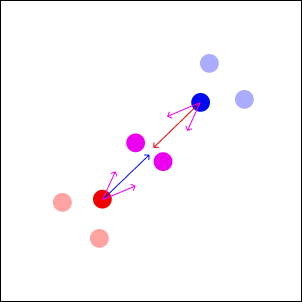
\includegraphics[height=0.4\textwidth]{images/collapse/Iteration 1 (1).png}
    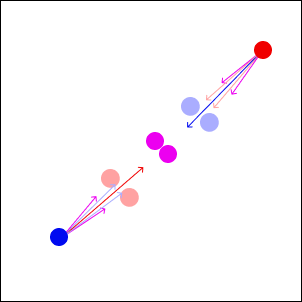
\includegraphics[height = 0.4\textwidth]{images/collapse/Iteration 2.png}

    \caption{One possible scenario leading to an exponential rise of velocity, illustrated by the positions of two neighbour data points (red and blue)  during two subsequent iterations and the key forces acting on them. The purple points are shared neighbours of red and blue while the lightly coloured red and blue points are non-shared neighbours. If force (\ref{tab:force}) is too strong, red and blue "overshoot" and end up on the opposite sides. The non-linearity in the applied force results from the additional forces acting on red and blue in the same direction. As the algorithm progresses, red and blue keep swapping sides moving further away from each other. At the same time, due to the strong forces, the points that do not "overshoot" tend to cluster together.}
    \label{fig:overshooting}
\end{figure}
The alternative of updating the positions of data points as soon as a force is calculated, instead of storing the cumulative force in $p_{u}$ was explored, but did not produce layouts of even vaguely adequate quality.

Nonetheless, it is important to note that the above is not intended as a comprehensive description of the system's behaviour during a "collapse" as this undoubtedly involves many complexities and variations not captured by the simple explanation given here and would require a much more in-depth investigation to describe fully.

\section{Hybrid algorithm corrections}









%==================================================================================================================================
\chapter{Implementation}
What did you do to implement this idea, and what technical achievements did you make?
\section{Guidance}
You can't talk about everything. Cover the high level first, then cover important, relevant or impressive details.

\section{General guidance for technical writing}

These points apply to the whole dissertation, not just this chapter.

\subsection{Figures}
\emph{Always} refer to figures included, like Figure \ref{fig:relu}, in the body of the text. Include full, explanatory captions and make sure the figures look good on the page.
You may include multiple figures in one float, as in Figure \ref{fig:synthetic}, using \texttt{subcaption}, which is enabled in the template.


% Figures are important. Use them well.
\begin{figure}[htb]
    \centering
    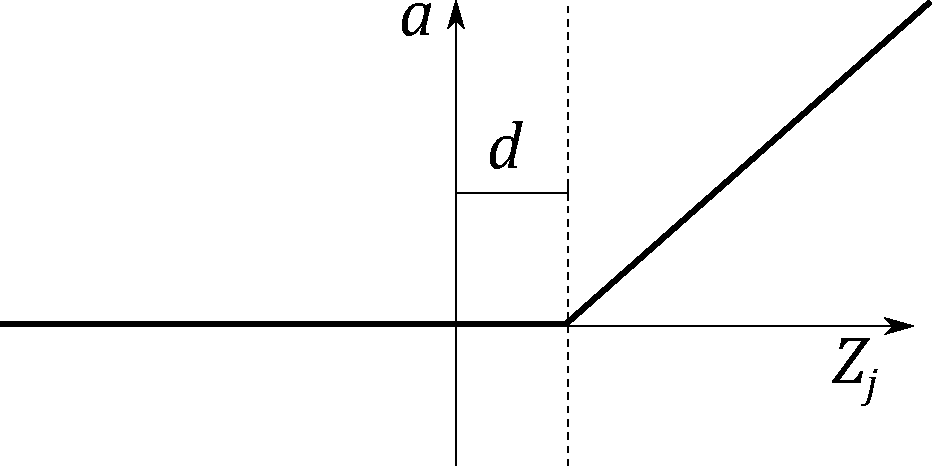
\includegraphics[width=0.5\linewidth]{images/relu.pdf}    

    \caption{In figure captions, explain what the reader is looking at: ``A schematic of the rectifying linear unit, where $a$ is the output amplitude,
    $d$ is a configurable dead-zone, and $Z_j$ is the input signal'', as well as why the reader is looking at this: 
    ``It is notable that there is no activation \emph{at all} below 0, which explains our initial results.'' 
    \textbf{Use vector image formats (.pdf) where possible}. Size figures appropriately, and do not make them over-large or too small to read.
    }

    % use the notation fig:name to cross reference a figure
    \label{fig:relu} 
\end{figure}


\begin{figure}[htb] 
    \centering
    \begin{subfigure}[b]{0.45\textwidth}
        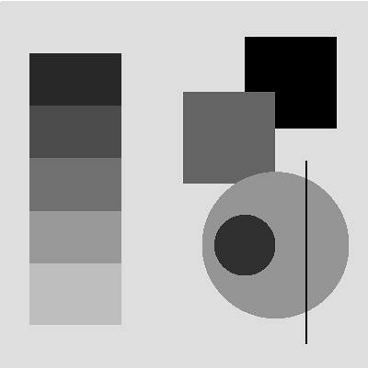
\includegraphics[width=\textwidth]{images/synthetic.png}
        \caption{Synthetic image, black on white.}
        \label{fig:syn1}
    \end{subfigure}
    ~ %add desired spacing between images, e. g. ~, \quad, \qquad, \hfill etc. 
      %(or a blank line to force the subfigure onto a new line)
    \begin{subfigure}[b]{0.45\textwidth}
        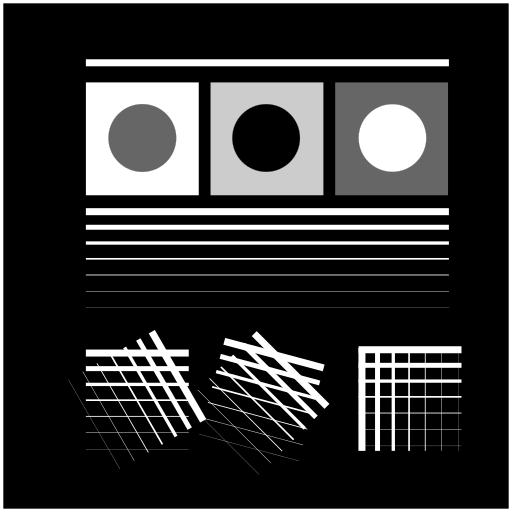
\includegraphics[width=\textwidth]{images/synthetic_2.png}
        \caption{Synthetic image, white on black.}
        \label{fig:syn2}
    \end{subfigure}
    ~ %add desired spacing between images, e. g. ~, \quad, \qquad, \hfill etc. 
    %(or a blank line to force the subfigure onto a new line)    
    \caption{Synthetic test images for edge detection algorithms. \subref{fig:syn1} shows various gray levels that require an adaptive algorithm. \subref{fig:syn2}
    shows more challenging edge detection tests that have crossing lines. Fusing these into full segments typically requires algorithms like the Hough transform.
    This is an example of using subfigures, with \texttt{subref}s in the caption.
    }\label{fig:synthetic}
\end{figure}

\clearpage

\subsection{Equations}

Equations should be typeset correctly and precisely. Make sure you get parenthesis sizing correct, and punctuate equations correctly 
(the comma is important and goes \textit{inside} the equation block). Explain any symbols used clearly if not defined earlier. 

For example, we might define:
\begin{equation}
    \hat{f}(\xi) = \frac{1}{2}\left[ \int_{-\infty}^{\infty} f(x) e^{2\pi i x \xi} \right],
\end{equation}    
where $\hat{f}(\xi)$ is the Fourier transform of the time domain signal $f(x)$.

\subsection{Algorithms}
Algorithms can be set using \texttt{algorithm2e}, as in Algorithm \ref{alg:metropolis}.

% NOTE: line ends are denoted by \; in algorithm2e
\begin{algorithm}
    \DontPrintSemicolon
    \KwData{$f_X(x)$, a probability density function returning the density at $x$.\; $\sigma$ a standard deviation specifying the spread of the proposal distribution.\;
    $x_0$, an initial starting condition.}
    \KwResult{$s=[x_1, x_2, \dots, x_n]$, $n$ samples approximately drawn from a distribution with PDF $f_X(x)$.}
    \Begin{
        $s \longleftarrow []$\;
        $p \longleftarrow f_X(x)$\;
        $i \longleftarrow 0$\;
        \While{$i < n$}
        {
            $x^\prime \longleftarrow \mathcal{N}(x, \sigma^2)$\;
            $p^\prime \longleftarrow f_X(x^\prime)$\;
            $a \longleftarrow \frac{p^\prime}{p}$\;
            $r \longleftarrow U(0,1)$\;
            \If{$r<a$}
            {
                $x \longleftarrow x^\prime$\;
                $p \longleftarrow f_X(x)$\;
                $i \longleftarrow i+1$\;
                append $x$ to $s$\;
            }
        }
    }
    
\caption{The Metropolis-Hastings MCMC algorithm for drawing samples from arbitrary probability distributions, 
specialised for normal proposal distributions $q(x^\prime|x) = \mathcal{N}(x, \sigma^2)$. The symmetry of the normal distribution means the acceptance rule takes the simplified form.}\label{alg:metropolis}
\end{algorithm}

\subsection{Tables}

If you need to include tables, like Table \ref{tab:operators}, use a tool like https://www.tablesgenerator.com/ to generate the table as it is
extremely tedious otherwise. 

\begin{table}[]
    \caption{The standard table of operators in Python, along with their functional equivalents from the \texttt{operator} package. Note that table
    captions go above the table, not below. Do not add additional rules/lines to tables. }\label{tab:operators}
    %\tt 
    \rowcolors{2}{}{gray!3}
    \begin{tabular}{@{}lll@{}}
    %\toprule
    \textbf{Operation}    & \textbf{Syntax}                & \textbf{Function}                            \\ %\midrule % optional rule for header
    Addition              & \texttt{a + b}                          & \texttt{add(a, b)}                                    \\
    Concatenation         & \texttt{seq1 + seq2}                    & \texttt{concat(seq1, seq2)}                           \\
    Containment Test      & \texttt{obj in seq}                     & \texttt{contains(seq, obj)}                           \\
    Division              & \texttt{a / b}                          & \texttt{div(a, b) }  \\
    Division              & \texttt{a / b}                          & \texttt{truediv(a, b) } \\
    Division              & \texttt{a // b}                         & \texttt{floordiv(a, b)}                               \\
    Bitwise And           & \texttt{a \& b}                         & \texttt{and\_(a, b)}                                  \\
    Bitwise Exclusive Or  & \texttt{a \textasciicircum b}           & \texttt{xor(a, b)}                                    \\
    Bitwise Inversion     & \texttt{$\sim$a}                        & \texttt{invert(a)}                                    \\
    Bitwise Or            & \texttt{a | b}                          & \texttt{or\_(a, b)}                                   \\
    Exponentiation        & \texttt{a ** b}                         & \texttt{pow(a, b)}                                    \\
    Identity              & \texttt{a is b}                         & \texttt{is\_(a, b)}                                   \\
    Identity              & \texttt{a is not b}                     & \texttt{is\_not(a, b)}                                \\
    Indexed Assignment    & \texttt{obj{[}k{]} = v}                 & \texttt{setitem(obj, k, v)}                           \\
    Indexed Deletion      & \texttt{del obj{[}k{]}}                 & \texttt{delitem(obj, k)}                              \\
    Indexing              & \texttt{obj{[}k{]}}                     & \texttt{getitem(obj, k)}                              \\
    Left Shift            & \texttt{a \textless{}\textless b}       & \texttt{lshift(a, b)}                                 \\
    Modulo                & \texttt{a \% b}                         & \texttt{mod(a, b)}                                    \\
    Multiplication        & \texttt{a * b}                          & \texttt{mul(a, b)}                                    \\
    Negation (Arithmetic) & \texttt{- a}                            & \texttt{neg(a)}                                       \\
    Negation (Logical)    & \texttt{not a}                          & \texttt{not\_(a)}                                     \\
    Positive              & \texttt{+ a}                            & \texttt{pos(a)}                                       \\
    Right Shift           & \texttt{a \textgreater{}\textgreater b} & \texttt{rshift(a, b)}                                 \\
    Sequence Repetition   & \texttt{seq * i}                        & \texttt{repeat(seq, i)}                               \\
    Slice Assignment      & \texttt{seq{[}i:j{]} = values}          & \texttt{setitem(seq, slice(i, j), values)}            \\
    Slice Deletion        & \texttt{del seq{[}i:j{]}}               & \texttt{delitem(seq, slice(i, j))}                    \\
    Slicing               & \texttt{seq{[}i:j{]}}                   & \texttt{getitem(seq, slice(i, j))}                    \\
    String Formatting     & \texttt{s \% obj}                       & \texttt{mod(s, obj)}                                  \\
    Subtraction           & \texttt{a - b}                          & \texttt{sub(a, b)}                                    \\
    Truth Test            & \texttt{obj}                            & \texttt{truth(obj)}                                   \\
    Ordering              & \texttt{a \textless b}                  & \texttt{lt(a, b)}                                     \\
    Ordering              & \texttt{a \textless{}= b}               & \texttt{le(a, b)}                                     \\
    % \bottomrule
    \end{tabular}
    \end{table}
\subsection{Code}

Avoid putting large blocks of code in the report (more than a page in one block, for example). Use syntax highlighting if possible, as in Listing \ref{lst:callahan}.

\begin{lstlisting}[language=python, float, caption={The algorithm for packing the $3\times 3$ outer-totalistic binary CA successor rule into a 
    $16\times 16\times 16\times 16$ 4 bit lookup table, running an equivalent, notionally 16-state $2\times 2$ CA.}, label=lst:callahan]
    def create_callahan_table(rule="b3s23"):
        """Generate the lookup table for the cells."""        
        s_table = np.zeros((16, 16, 16, 16), dtype=np.uint8)
        birth, survive = parse_rule(rule)

        # generate all 16 bit strings
        for iv in range(65536):
            bv = [(iv >> z) & 1 for z in range(16)]
            a, b, c, d, e, f, g, h, i, j, k, l, m, n, o, p = bv

            # compute next state of the inner 2x2
            nw = apply_rule(f, a, b, c, e, g, i, j, k)
            ne = apply_rule(g, b, c, d, f, h, j, k, l)
            sw = apply_rule(j, e, f, g, i, k, m, n, o)
            se = apply_rule(k, f, g, h, j, l, n, o, p)

            # compute the index of this 4x4
            nw_code = a | (b << 1) | (e << 2) | (f << 3)
            ne_code = c | (d << 1) | (g << 2) | (h << 3)
            sw_code = i | (j << 1) | (m << 2) | (n << 3)
            se_code = k | (l << 1) | (o << 2) | (p << 3)

            # compute the state for the 2x2
            next_code = nw | (ne << 1) | (sw << 2) | (se << 3)

            # get the 4x4 index, and write into the table
            s_table[nw_code, ne_code, sw_code, se_code] = next_code

        return s_table

\end{lstlisting}

%==================================================================================================================================
\chapter{Evaluation} 
How good is your solution? How well did you solve the general problem, and what evidence do you have to support that?

\section{Guidance}
\begin{itemize}
    \item
        Ask specific questions that address the general problem.
    \item
        Answer them with precise evidence (graphs, numbers, statistical
        analysis, qualitative analysis).
    \item
        Be fair and be scientific.
    \item
        The key thing is to show that you know how to evaluate your work, not
        that your work is the most amazing product ever.
\end{itemize}

\section{Evidence}
Make sure you present your evidence well. Use appropriate visualisations, 
reporting techniques and statistical analysis, as appropriate. The point is not
to dump all the data you have but to present an argument well supported by evidence gathered.

If you use numerical evidence, specify reasonable numbers of significant digits; don't state ``18.41141\% of users were successful'' if you only had 20 users. If you average \textit{anything}, present both a measure of central tendency (e.g. mean, median) \textit{and} a measure of spread (e.g. standard deviation, min/max, interquartile range).

You can use \texttt{siunitx} to define units, space numbers neatly, and set the precision for the whole LaTeX document. 

% setup siunitx to have two decimal places
\sisetup{
	round-mode = places,
	round-precision = 2
}

For example, these numbers will appear with two decimal places: \num{3.141592}, \num{2.71828}, and this one will appear with reasonable spacing \num{1000000}.



If you use statistical procedures, make sure you understand the process you are using,
and that you check the required assumptions hold in your case. 

If you visualise, follow the basic rules, as illustrated in Figure \ref{fig:boxplot}:
\begin{itemize}
\item Label everything correctly (axis, title, units).
\item Caption thoroughly.
\item Reference in text.
\item \textbf{Include appropriate display of uncertainty (e.g. error bars, Box plot)}
\item Minimize clutter.
\end{itemize}

See the file \texttt{guide\_to\_visualising.pdf} for further information and guidance.

\begin{figure}[htb]
    \centering
    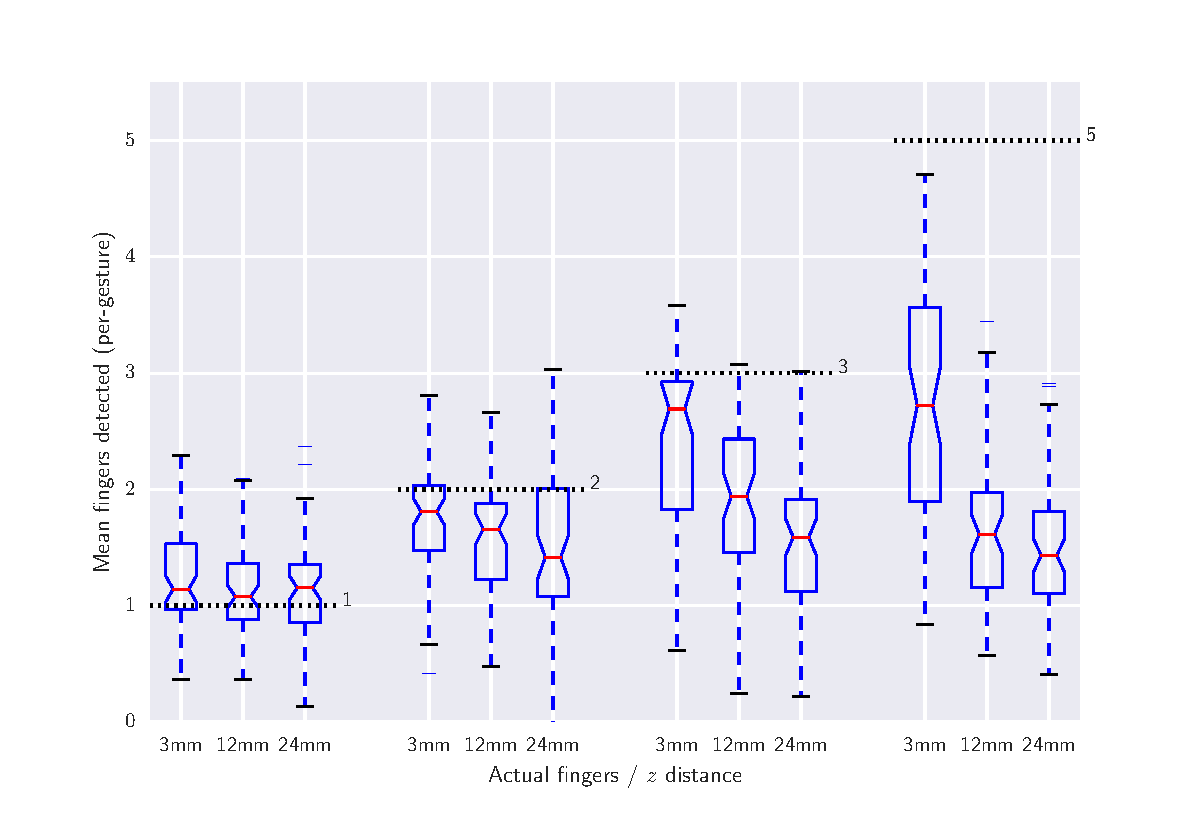
\includegraphics[width=1.0\linewidth]{images/boxplot_finger_distance.pdf}    

    \caption{Average number of fingers detected by the touch sensor at different heights above the surface, averaged over all gestures. Dashed lines indicate
    the true number of fingers present. The Box plots include bootstrapped uncertainty notches for the median. It is clear that the device is biased toward 
    undercounting fingers, particularly at higher $z$ distances.
    }

    % use the notation fig:name to cross reference a figure
    \label{fig:boxplot} 
\end{figure}


%==================================================================================================================================
\chapter{Conclusion}    
Summarise the whole project for a lazy reader who didn't read the rest (e.g. a prize-awarding committee). This chapter should be short in most dissertations; maybe one to three pages.
\section{Guidance}
\begin{itemize}
    \item
        Summarise briefly and fairly.
    \item
        You should be addressing the general problem you introduced in the
        Introduction.        
    \item
        Include summary of concrete results (``the new compiler ran 2x
        faster'')
    \item
        Indicate what future work could be done, but remember: \textbf{you
        won't get credit for things you haven't done}.
\end{itemize}

\section{Summary}
Summarise what you did; answer the general questions you asked in the introduction. What did you achieve? Briefly describe what was built and summarise the evaluation results.

\section{Reflection}
Discuss what went well and what didn't and how you would do things differently if you did this project again.

\section{Future work}
Discuss what you would do if you could take this further -- where would the interesting directions to go next be? (e.g. you got another year to work on it, or you started a company to work on this, or you pursued a PhD on this topic)

%==================================================================================================================================
%
% 
%==================================================================================================================================
%  APPENDICES  

\begin{appendices}


\chapter{Appendix A}
\label{appendix a}

\begin{figure}[htb]
    \centering
    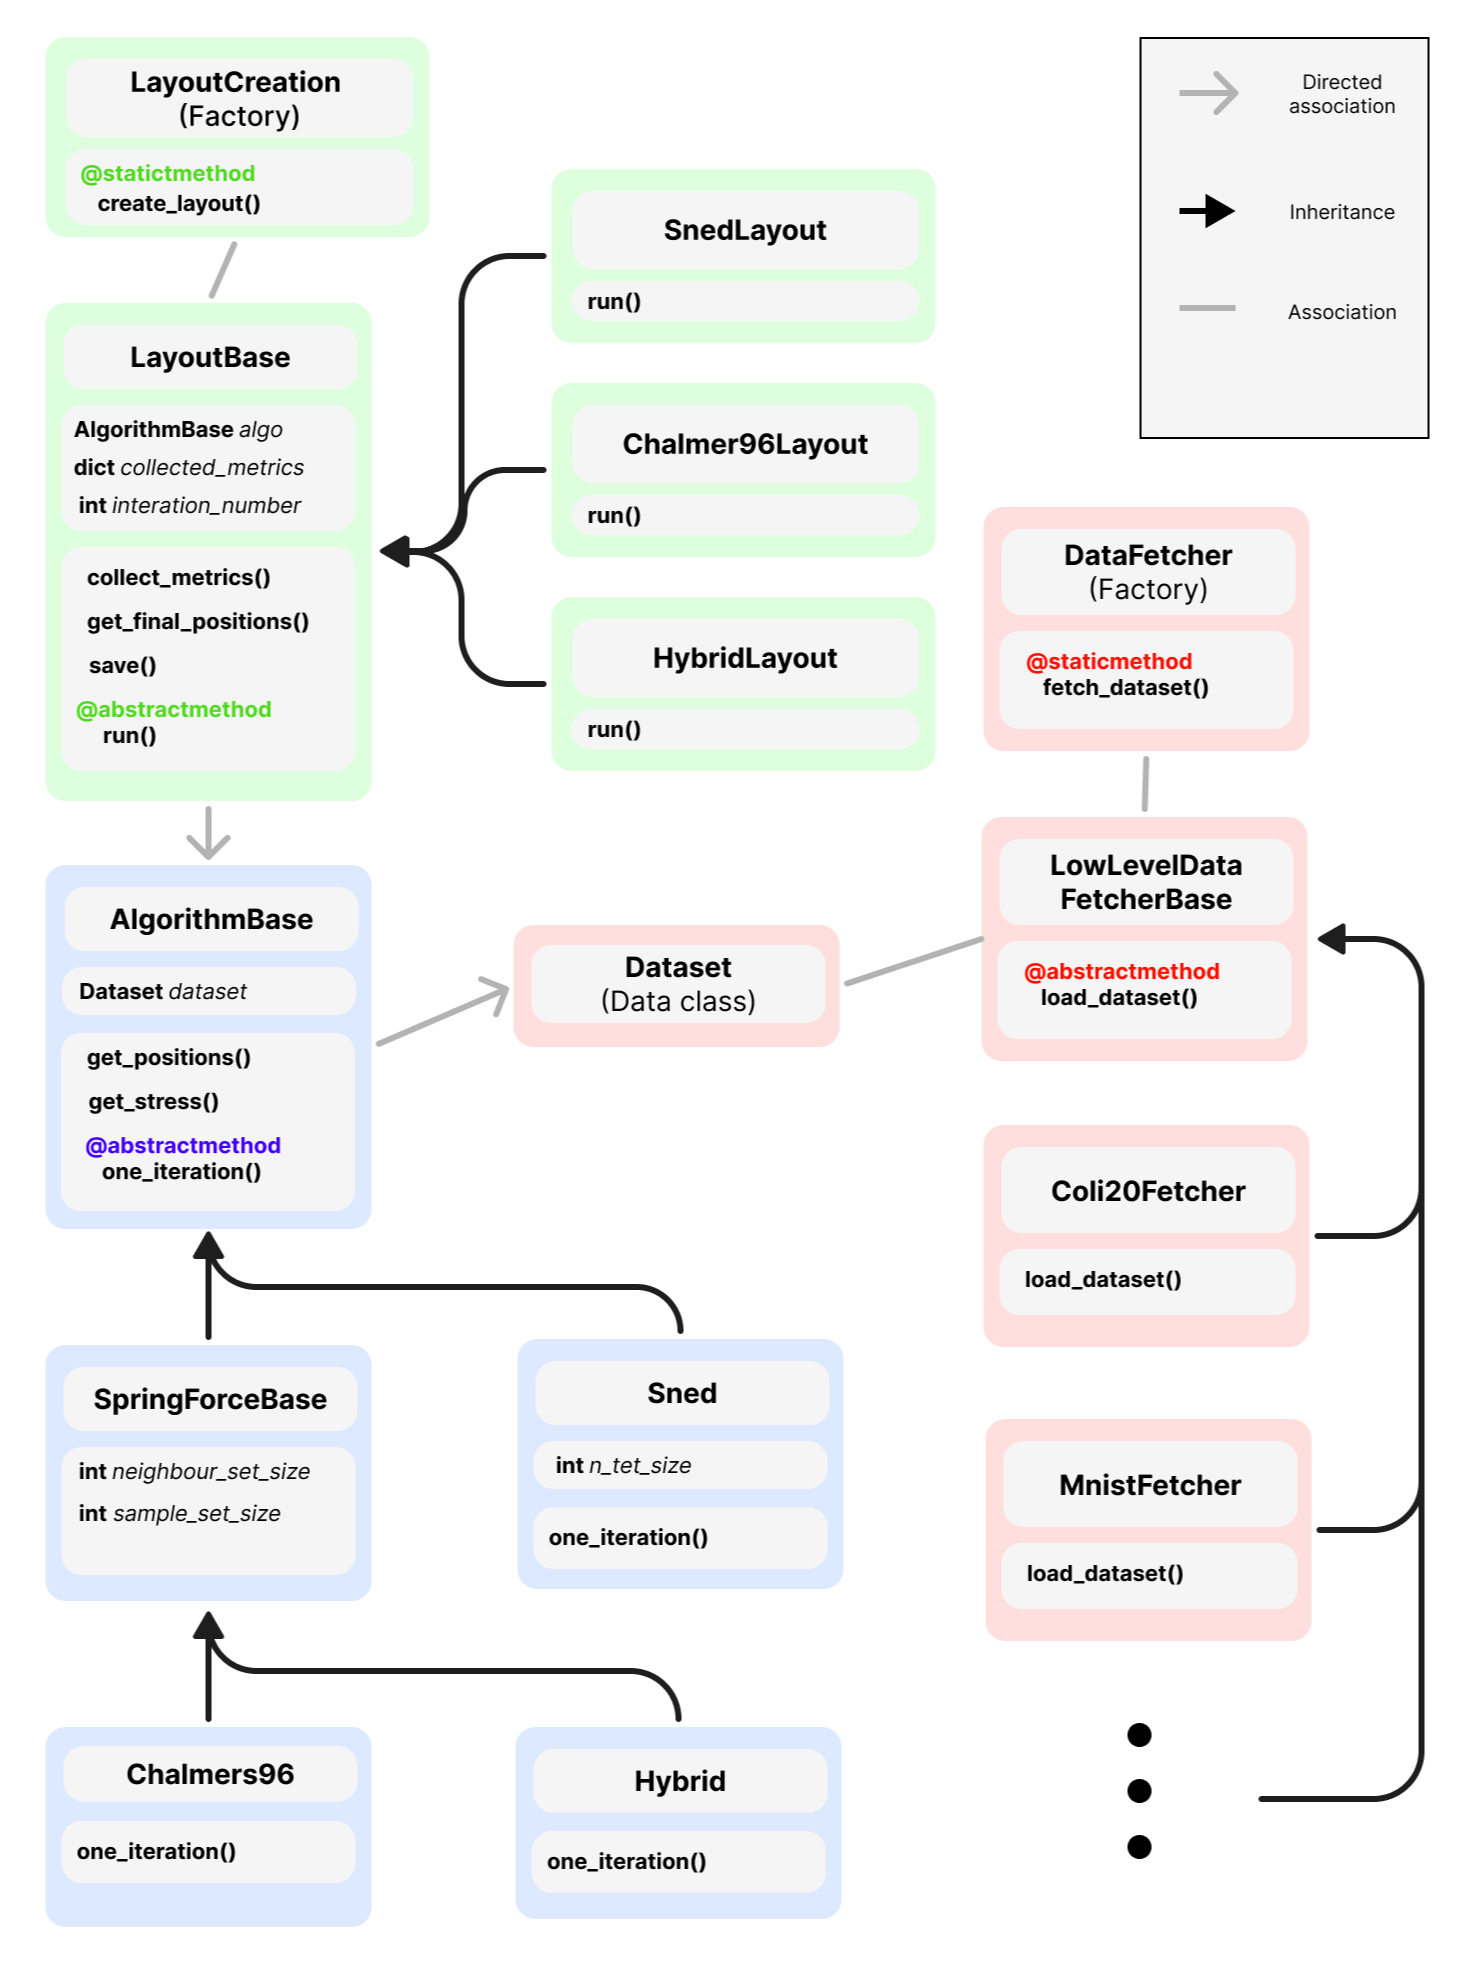
\includegraphics[width=1\linewidth]{images/class diag.png} \\
 
    \caption{A simplified class diagram for the project showing the key classes and the separation of concerns. Red classes are responsible for data pre-processing and loading, blue contain the main logic of all algorithms and green create layouts as well as collect various measurements during the process.
    }

    % use the notation fig:name to cross reference a figure
    \label{fig:uml} 
\end{figure}

\chapter{Appendix B}
\label{appendix b}

\begin{figure}[ht]
\centering
    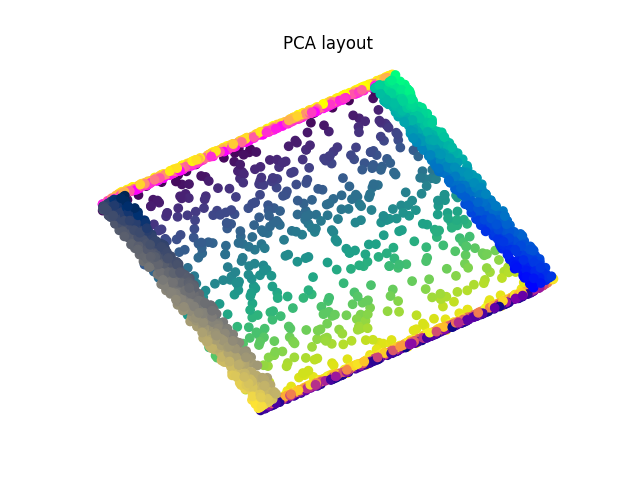
\includegraphics[width=0.4\linewidth]{images/n-tet layouts/cube/PCA layout.png} 
    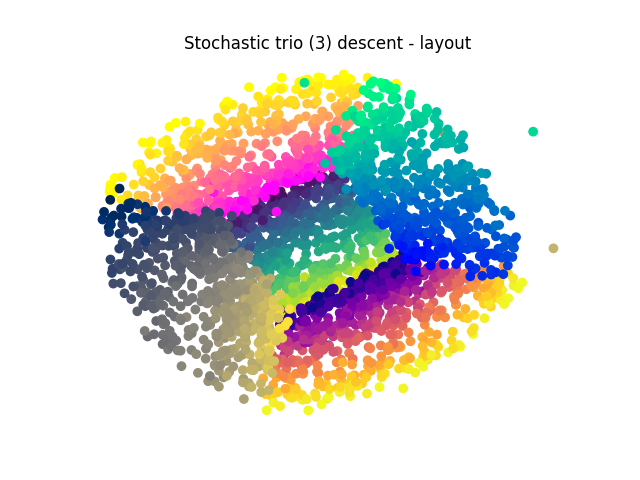
\includegraphics[width=0.4\linewidth]{images/n-tet layouts/cube/Stochastic trio (3) descent - layout.png} \\
    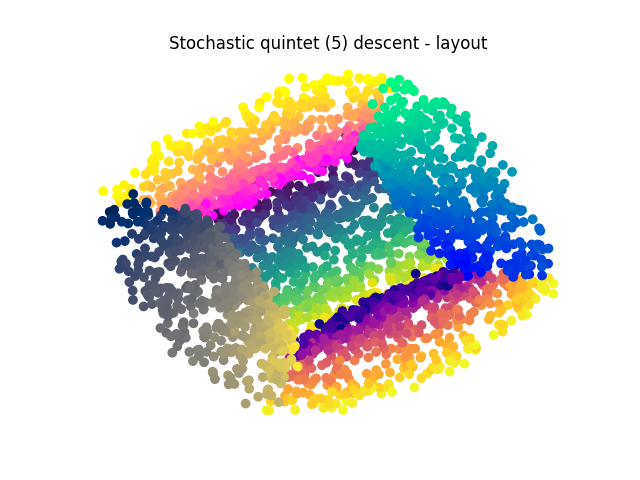
\includegraphics[width=0.4\linewidth]{images/n-tet layouts/cube/Stochastic quintet (5) descent - layout.png}
    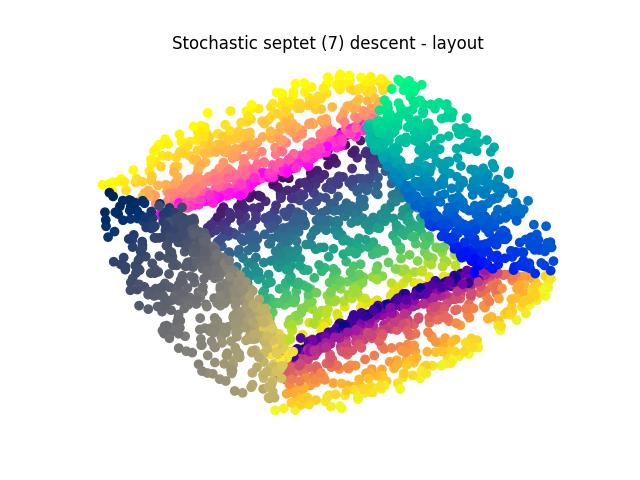
\includegraphics[width=0.4\linewidth]{images/n-tet layouts/cube/Stochastic septet (7) descent - layout.png} \\
    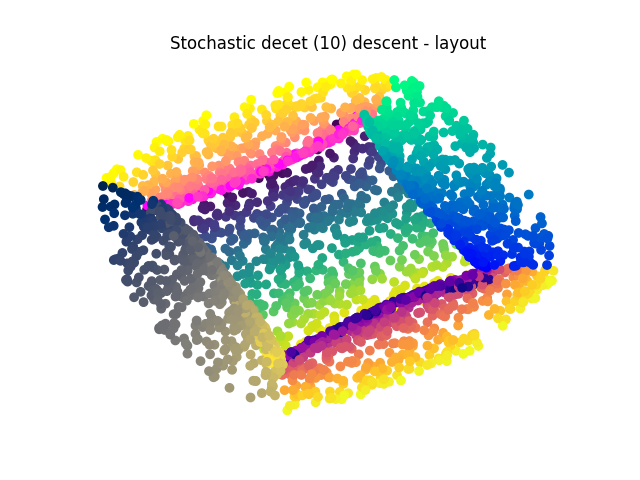
\includegraphics[width=0.4\linewidth]{images/n-tet layouts/cube/Stochastic decet (10) descent - layout.png} 
    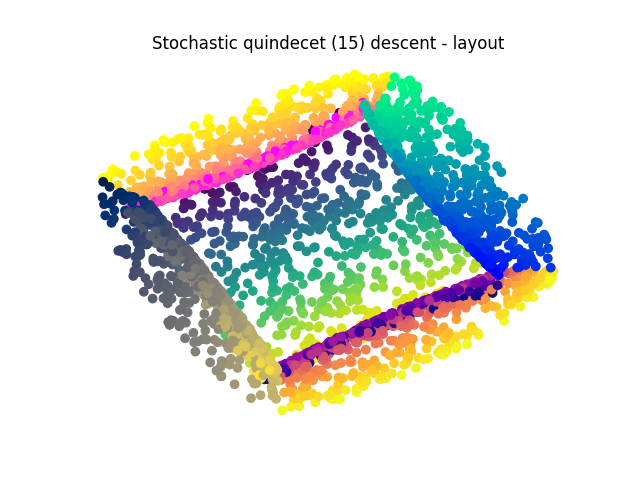
\includegraphics[width=0.4\linewidth]{images/n-tet layouts/cube/Stochastic quindecet (15) descent - layout.png}\\
    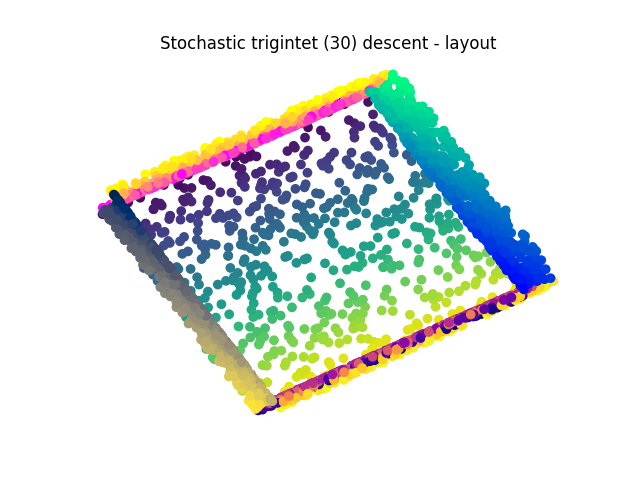
\includegraphics[width=0.4\linewidth]{images/n-tet layouts/cube/Stochastic trigintet (30) descent - layout.png} 
    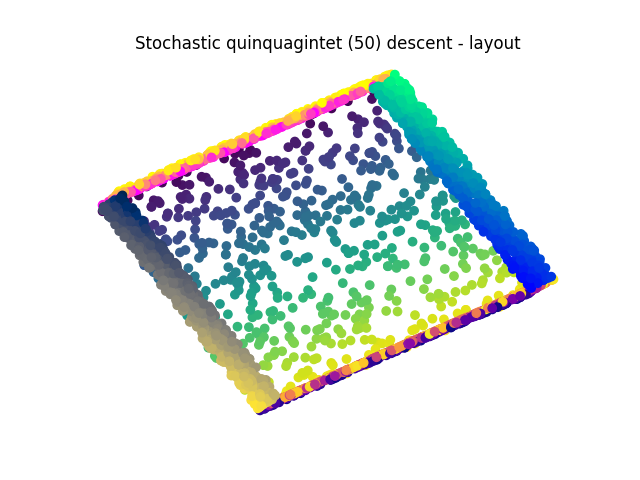
\includegraphics[width=0.4\linewidth]{images/n-tet layouts/cube/Stochastic quinquagintet (50) descent - layout.png} \\


    \caption{Resulting layouts/embeddings of the Cube dataset after 1000 iterations of the SNeD algorithm for different n-tet sizes.
    }

    % use the notation fig:name to cross reference a figure
    \label{fig:init_demo} 
\end{figure}


\begin{figure}[ht]
\centering
    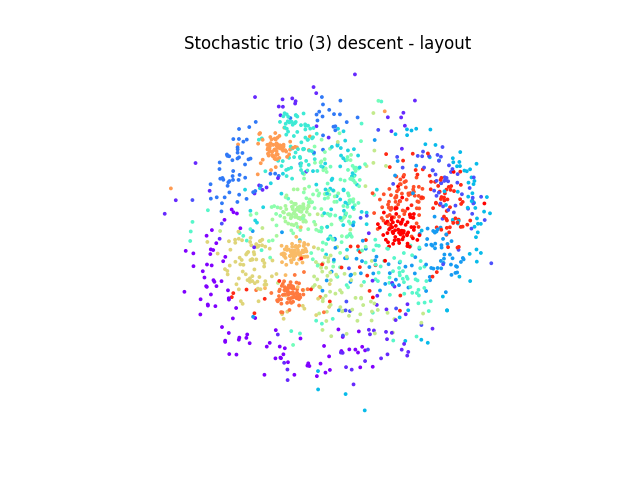
\includegraphics[width=0.4\linewidth]{images/n-tet layouts/coil20/Stochastic trio (3) descent - layout.png} 
    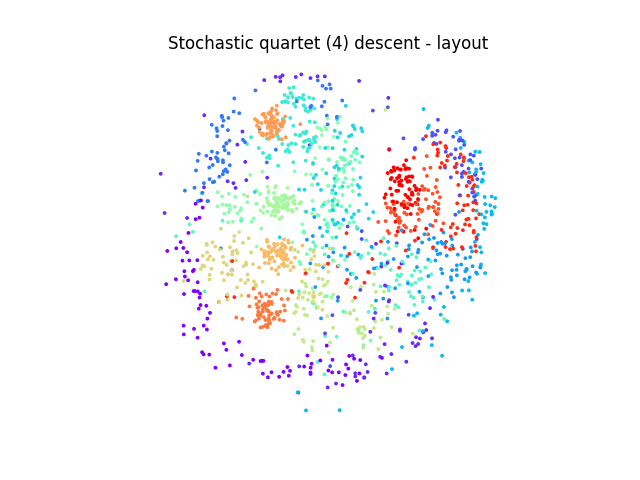
\includegraphics[width=0.4\linewidth]{images/n-tet layouts/coil20/Stochastic quartet (4) descent - layout.png}\\
    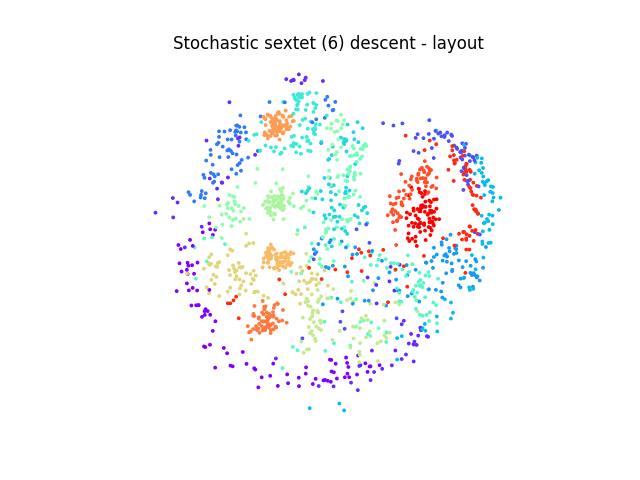
\includegraphics[width=0.4\linewidth]{images/n-tet layouts/coil20/Stochastic sextet (6) descent - layout.png} 
    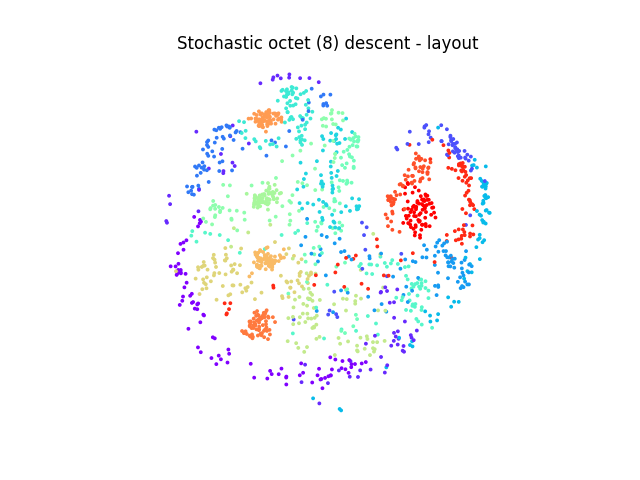
\includegraphics[width=0.4\linewidth]{images/n-tet layouts/coil20/Stochastic octet (8) descent - layout.png}\\
    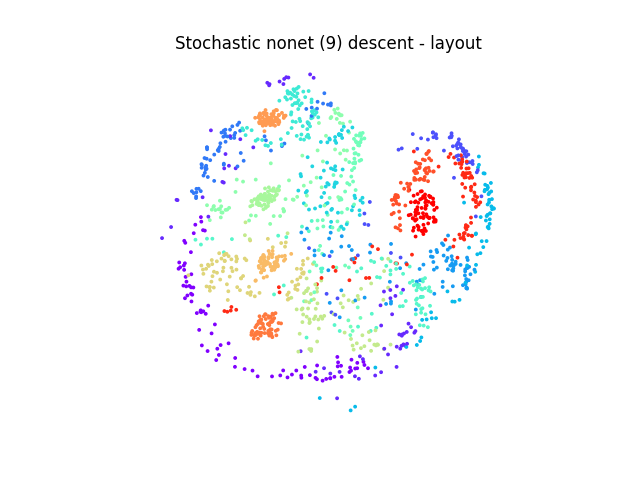
\includegraphics[width=0.4\linewidth]{images/n-tet layouts/coil20/Stochastic nonet (9) descent - layout.png} 
    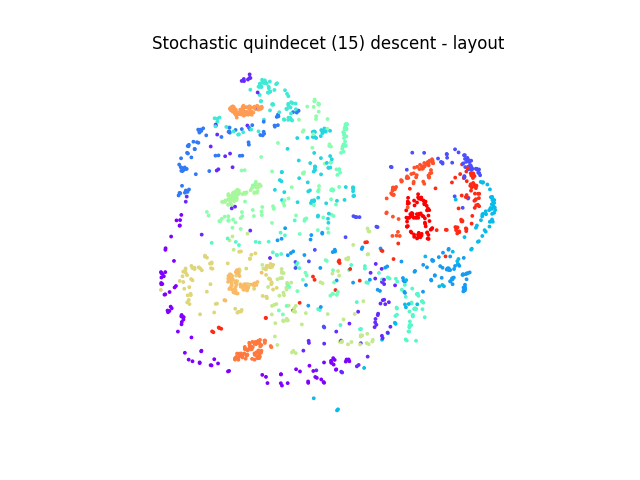
\includegraphics[width=0.4\linewidth]{images/n-tet layouts/coil20/Stochastic quindecet (15) descent - layout.png} \\
    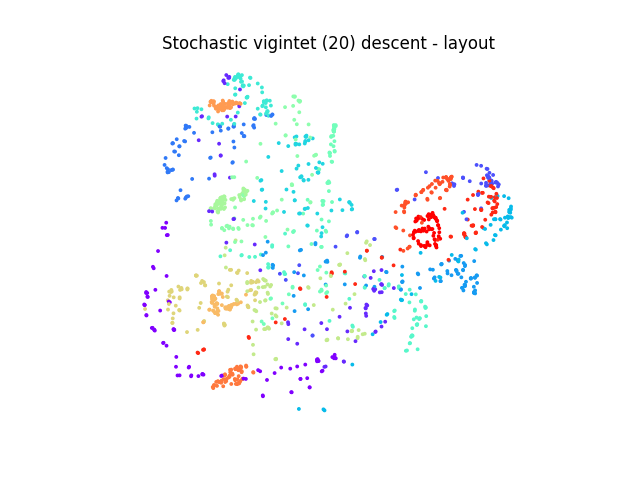
\includegraphics[width=0.4\linewidth]{images/n-tet layouts/coil20/Stochastic vigintet (20) descent - layout.png}
    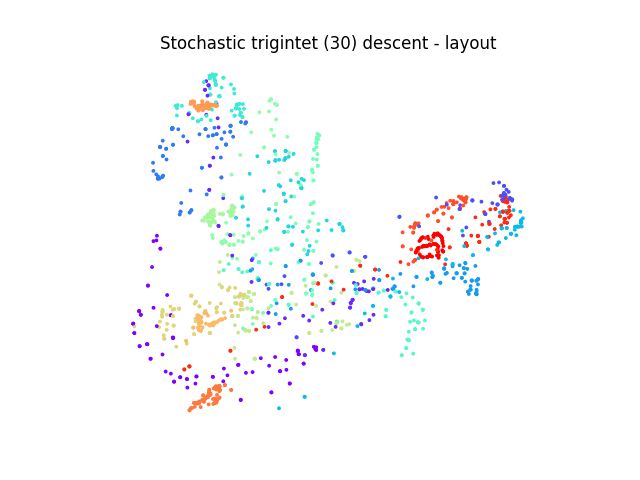
\includegraphics[width=0.4\linewidth]{images/n-tet layouts/coil20/Stochastic trigintet (30) descent - layout.png} \\
    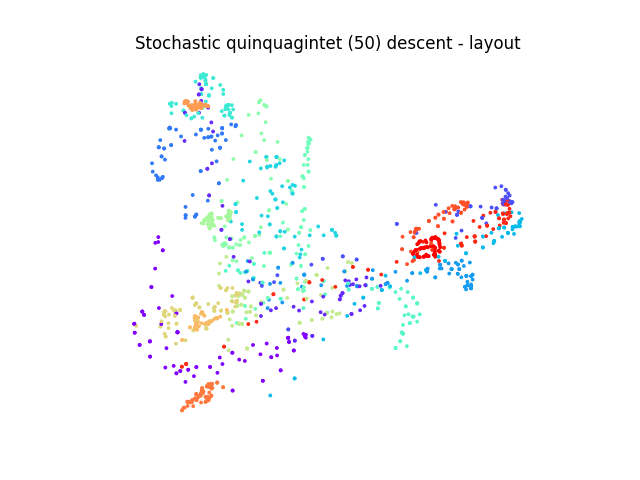
\includegraphics[width=0.4\linewidth]{images/n-tet layouts/coil20/Stochastic quinquagintet (50) descent - layout.png} 
    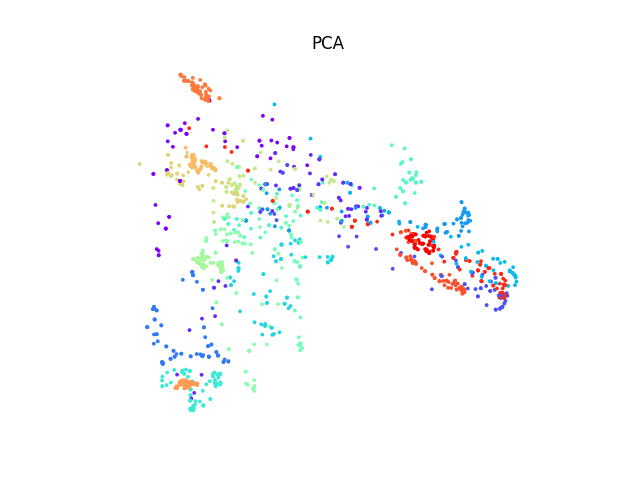
\includegraphics[width=0.4\linewidth]{images/n-tet layouts/coil20/PCA.png}


    \caption{Resulting layouts/embeddings of the Coli20 dataset after 1000 iterations of the SNeD algorithm for different n-tet sizes, coloured by their true labels. Similarly to the other datasets, the layout for n-tet size 50 appears indistinguishable from that produced by PCA
    }

    % use the notation fig:name to cross reference a figure
    \label{fig:init_demo} 
\end{figure}


\begin{figure}[ht]
\centering
    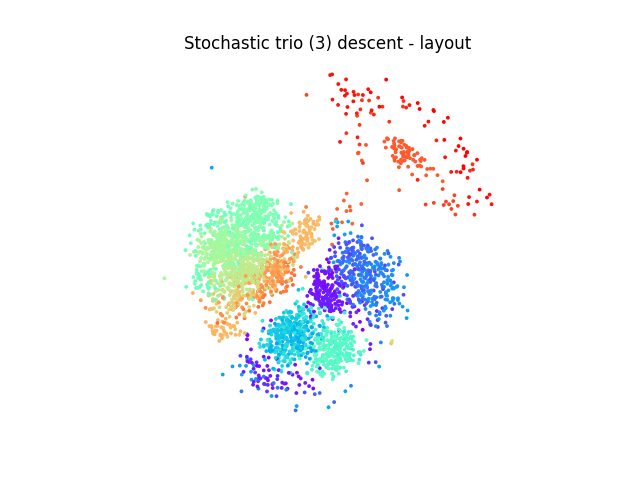
\includegraphics[width=0.4\linewidth]{images/n-tet layouts/mouse RNA/Stochastic trio (3) descent - layout.png} 
    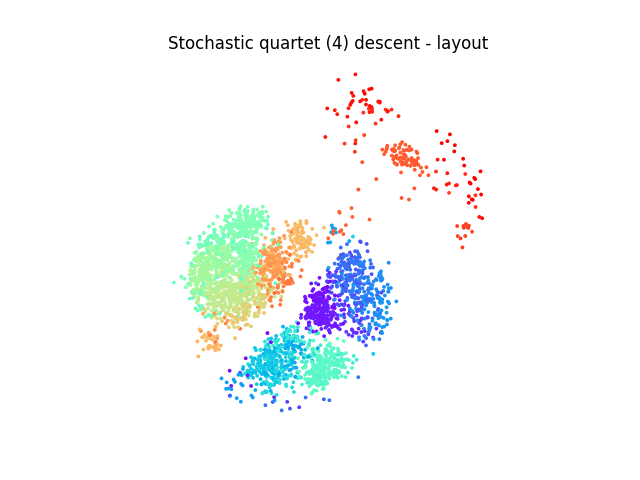
\includegraphics[width=0.4\linewidth]{images/n-tet layouts/mouse RNA/Stochastic quartet (4) descent - layout.png}\\
    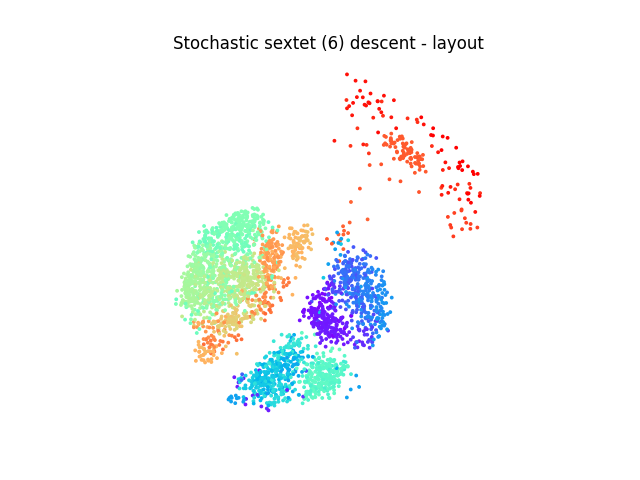
\includegraphics[width=0.4\linewidth]{images/n-tet layouts/mouse RNA/Stochastic sextet (6) descent - layout.png} 
    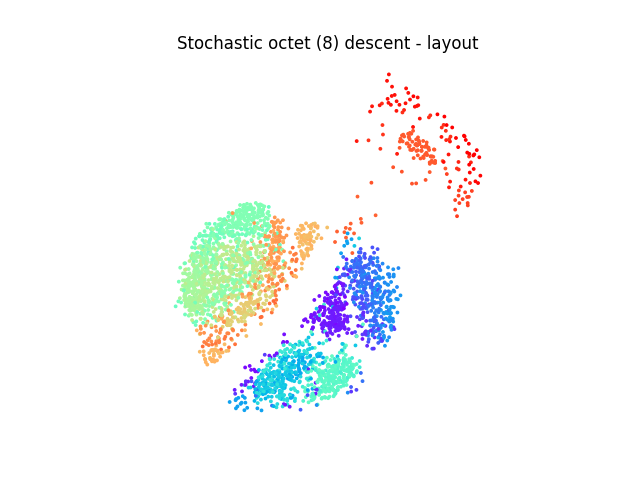
\includegraphics[width=0.4\linewidth]{images/n-tet layouts/mouse RNA/Stochastic octet (8) descent - layout.png}\\
    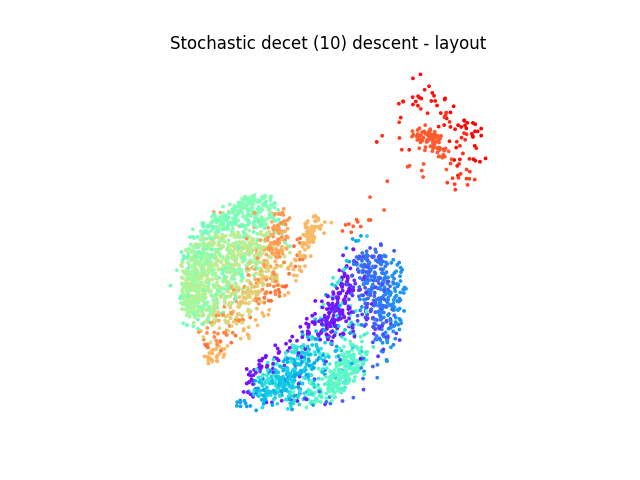
\includegraphics[width=0.4\linewidth]{images/n-tet layouts/mouse RNA/Stochastic decet (10) descent - layout.png} 
    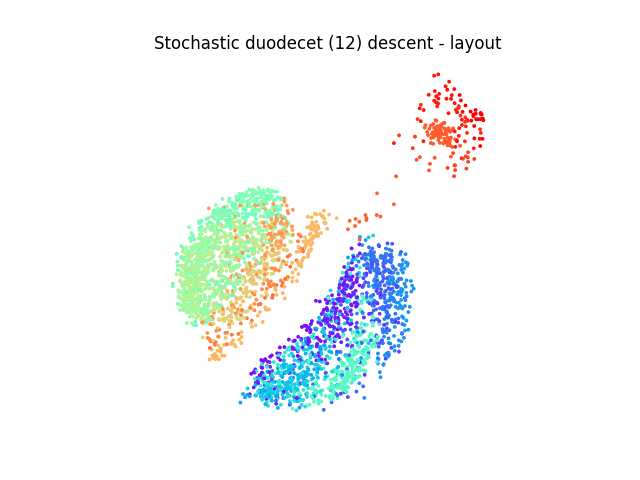
\includegraphics[width=0.4\linewidth]{images/n-tet layouts/mouse RNA/Stochastic duodecet (12) descent - layout.png} \\
    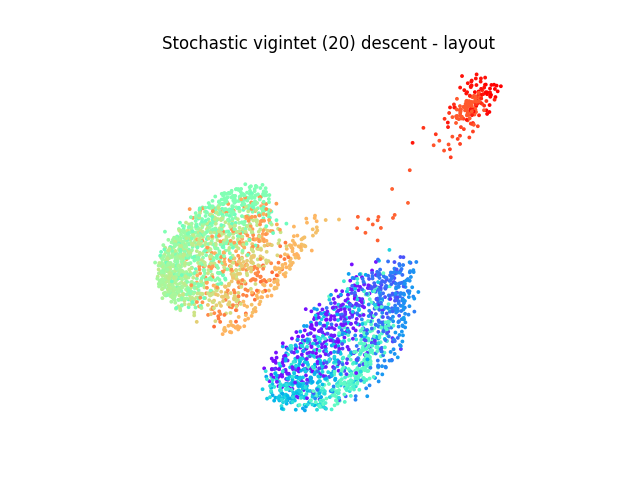
\includegraphics[width=0.4\linewidth]{images/n-tet layouts/mouse RNA/Stochastic vigintet (20) descent - layout.png}
    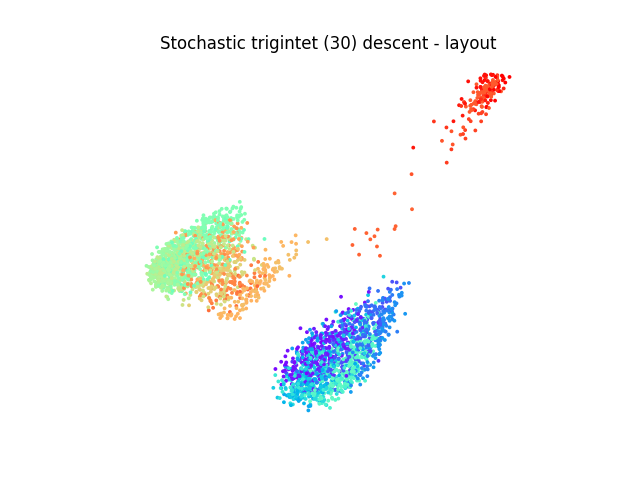
\includegraphics[width=0.4\linewidth]{images/n-tet layouts/mouse RNA/Stochastic trigintet (30) descent - layout.png} \\
    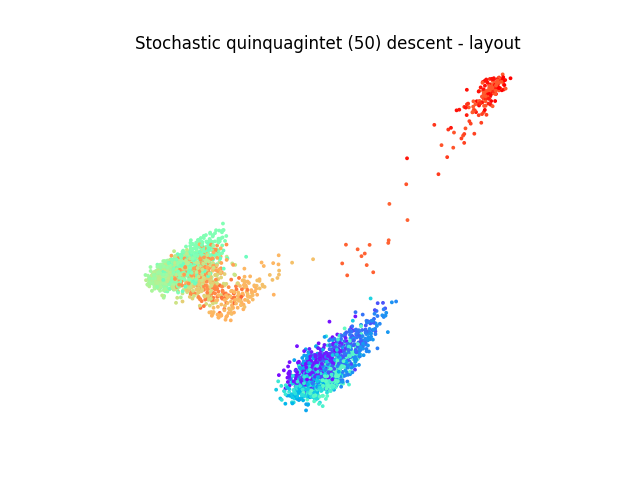
\includegraphics[width=0.4\linewidth]{images/n-tet layouts/mouse RNA/Stochastic quinquagintet (50) descent - layout.png} 
    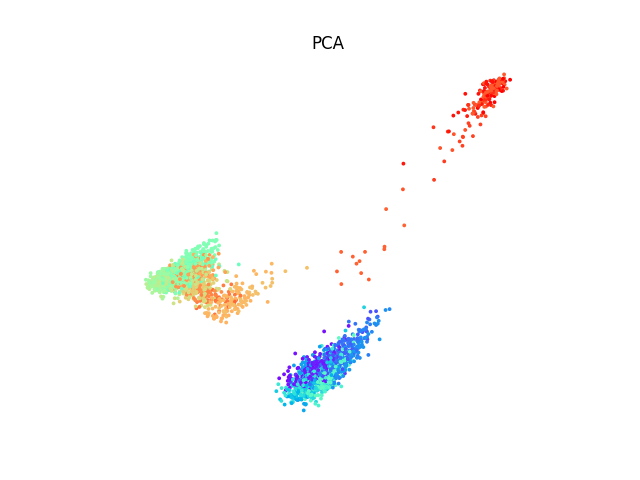
\includegraphics[width=0.4\linewidth]{images/n-tet layouts/mouse RNA/pca.png}
    
    


    \caption{Resulting layouts/embeddings of the Mouse cortex scRNA dataset after 1000 iterations of the SNeD algorithm for different n-tet sizes, coloured by their true labels. Similarly to the other datasets, the layout for n-tet size 50 appears indistinguishable from that produced by PCA.
    }

    % use the notation fig:name to cross reference a figure
    \label{fig:init_demo} 
\end{figure}


\chapter{Appendix C}
\label{appendix c}

\begin{figure}[htb]
    \centering
    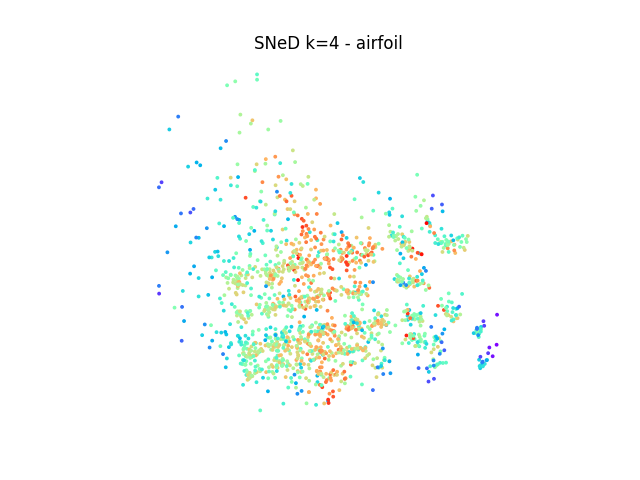
\includegraphics[width=0.4\linewidth]{images/tsne_umap_compare/airfoilsned.png} 
    \includegraphics[width=0.4\linewidth]{images/tsne_umap_compare/sned_shuttle.png}\\
    \includegraphics[width=0.4\linewidth]{images/tsne_umap_compare/airfoli96.png} 
    \includegraphics[width=0.4\linewidth]{images/tsne_umap_compare/shuttle_96.png}\\
    \includegraphics[width=0.4\linewidth]{images/tsne_umap_compare/tsneairfoil.png} 
    \includegraphics[width=0.4\linewidth]{images/tsne_umap_compare/tsne_shuttle.png} \\
    \includegraphics[width=0.4\linewidth]{images/tsne_umap_compare/umapairfoil.png}
    \includegraphics[width=0.4\linewidth]{images/tsne_umap_compare/umap_shuttle.png} \\



    \caption{ Airfoil dataset\footnote{\url{https://archive.ics.uci.edu/ml/datasets/airfoil\+self-noise}} and Shuttle data set\footnote{\url{https://archive.ics.uci.edu/ml/datasets/Statlog\-(Shuttle)}}
    }

    % use the notation fig:name to cross reference a figure
    \label{fig:init_demo} 
\end{figure}

\chapter{Appendix D}
\label{appendix d}

\begin{table}[ht]
\centering
\begin{tabular}{|
>{\columncolor[HTML]{DAE8FC}}l |c|c|c|}
\hline
\multicolumn{1}{|c|}{\cellcolor[HTML]{CBCEFB}} &
  \cellcolor[HTML]{CBCEFB}\begin{tabular}[c]{@{}c@{}}kNND Mean \\ execution time (s)\end{tabular} &
  \cellcolor[HTML]{CBCEFB}\begin{tabular}[c]{@{}c@{}}Mean execution time \\ without kNND (s)\end{tabular} &
  \cellcolor[HTML]{CBCEFB}\begin{tabular}[c]{@{}c@{}}Welch's t-test \\ p-value\end{tabular} \\ \hline
Mouse cortex scRNA & 64.13 (SD 0.5)   & 83.64 (SD 0.48)   & 1.31e-62 \\ \hline
Coli20             & 34.08 (SD 0.82)  & 46.19  (SD 0.25)  & 1.11e-33 \\ \hline
Globe              & 170.79 (SD 4.17) & 197.21 (SD 7.49)  & 7.62e-18 \\ \hline
Fashion mnist      & 204.42 (SD 2.31) & 233.94 (SD  1.03) & 4.86e-35 \\ \hline
Mnist              & 215.62 (SD 6.51) & 236.99 (SD 11.38) & 5.77e-10 \\ \hline
\end{tabular}
\caption{Summary of the results of running the Chalmers' 96 algorithm 25 for each condition (with and without applying kNND) for each data set, with execution time measured in seconds. The Welch's test used the alternative hypotesis of the mean without kNND being greater.}
\label{tab:knnd times}
\end{table}


\chapter{Appendices}

Use separate appendix chapters for groups of ancillary material that support your dissertation. 
Typical inclusions in the appendices are:

\begin{itemize}
\item
  Copies of ethics approvals (you must include these if you needed to get them)
\item
  Copies of questionnaires etc. used to gather data from subjects. Don't include
  voluminous data logs; instead submit these electronically alongside your source code.
\item
  Extensive tables or figures that are too bulky to fit in the main body of
  the report, particularly ones that are repetitive and summarised in the body.
\item Outline of the source code (e.g. directory structure), 
    or other architecture documentation like class diagrams.
\item User manuals, and any guides to starting/running the software. 
Your equivalent of \texttt{readme.md} should be included.

\end{itemize}

\textbf{Don't include your source code in the appendices}. It will be
submitted separately.



\end{appendices}

%==================================================================================================================================
%   BIBLIOGRAPHY   

% The bibliography style is agsm (Harvard)
% The bibliography always appears last, after the appendices.

\bibliographystyle{agsm}

% Force the bibliography not to be numbered
\renewcommand{\thechapter}{0} 
\bibliography{l4proj}

\end{document}
